\chapter{Learning uncertainty tubes via recurrent neural networks} \label{chap:NN}
\markboth{Learning uncertainty tubes via recurrent neural networks}{}% To set left/right header
\localtableofcontents \newpage

This chapter introduces the second major contribution of this thesis: a deep learning approach for rapidly and accurately estimating sensitivity-based uncertainty tubes. 
As demonstrated in Chapter~\ref{chap:samp}, the computation of such tubes using \myglsentry{odes} considerably reduces the efficiency of sampling-based methods, particularly for complex systems.
To overcome this limitation, this chapter introduces a method based on \gls{rnns} to eliminate the dependency on solving \myglsentry{odes}.
By leveraging structural similarities between \myglsentry{odes} and \myglsentry{rnns}, the proposed neural network architecture achieves significantly faster predictions of uncertainty tubes compared to traditional solvers, thereby improving computational efficiency while maintaining accuracy.

This chapter is organized as follows: Section~\ref{sec:learning_overview} begins with an overview of parallelization techniques for \myglsentry{odes} and learning methods for \myglsentry{odes}.
Section~\ref{sec:method} details the proposed method, including the neural network architecture and dataset generation process. 
Evaluation metrics, training procedures, and implementation details are discussed in Section~\ref{sec:nn_eval}. 
Finally, Section~\ref{sec:nn_results} presents the results for the quadrotor and differential drive robot, while Section~\ref{sec:concl} concludes the chapter.

For clarity, in the following sections of this chapter, methods are referred to in non-bold, and models are referred to in bold (e.g., \textbf{GRU} refers to the proposed GRU-based architecture, and GRU refers to the Gated Recurrent Unit method).

% This chapter is associated to the following publication in ECAI 2024~\cite{cECAI}: Wasiela, S., Bouhsain, S. A., Cognetti, M., Cortés, J., and Simeon, T. (2024, October). "Learned Uncertainty Tubes via Recurrent Neural Networks for Planning Robust Robot Motions." In 27th European Conference on Artificial Intelligence (ECAI) (pp. 4385-4392).\footnote{The results presented in this chapter slightly differ from those in the article due to improvements in implementation.}

\section{Related work}\label{sec:learning_overview}

This section begins with an overview of parallelization techniques for \myglsentry{odes}, such as the Parareal algorithm~\cite{cParareal}, which aims to accelerate computations by distributing the workload across multiple processors. 
It then explores learning approaches related to \myglsentry{odes}, including \gls{pinns} and NeuralODEs, which incorporate the structure and dynamics of differential equations into the learning process. 
Finally, the section introduces \myglsentry{rnns}, emphasizing their structural similarities to \myglsentry{odes} and their potential for efficiently modeling temporal and sequential data in the context of dynamical systems.

The set of \myglsentry{odes} that has to be computationally speed up has the following intrinsic structure within a single time step: Equation~(\ref{eq:ctrl}) computes the control inputs, Equation~(\ref{eq:dyna}) updates the robot state, and Equation~(\ref{eq:dyna_sensi}) computes the sensitivity matrices before projecting them to derive the uncertainty tubes (see Equation~(\ref{eq:radius})). 

\subsection{ODEs parallelization}

This subsection discusses various techniques used to parallelize the computation of \myglsentry{odes}, such as the Parareal algorithm~\cite{cParareal}, which divides the solution process into multiple steps to be processed in parallel, improving efficiency.

\begin{itemize}
    \item The first and most straightforward approach to parallelizing the \myglsentry{odes} is to compute each equation in parallel across different threads, exploiting the decoupling between the equations. 
    However, in the current set, each equation depends on the outputs of the preceding one within a single time step.
    Additionally, certain robot dynamics exhibit inherent coupling (e.g., for a quadrotor).
    These dependencies make parallelization inefficient in this context, as the computation cannot be fully decoupled across threads. 
    \item Another well-known method for parallelizing the computation of \myglsentry{odes} is the Parareal algorithm~\cite{cParareal}.
    The approach involves dividing the time domain into smaller intervals, which can then be computed in parallel using different processors for each interval. 
    The Parareal algorithm works by initially approximating the solution of each sub-interval using a coarse solver, followed by a more accurate fine solver that is applied in parallel. 
    The iterative process allows the fine solver to correct discrepancies between the coarse solutions, ultimately improving the overall accuracy of the solution.
    However, its effectiveness can be limited by the coupling between different parts of the \myglsentry{odes}, as seen in the current case.
    This coupling limits the potential for Parareal method.
    Furthermore, since the current case involves control application, the first step of the algorithm, which consist of a coarse solver, might struggle to converge to a sufficiently accurate solution, making it difficult to refine it further in subsequent iterations.
\end{itemize}

While \myglsentry{odes} parallelization methods can be useful for speeding up large-scale simulations or off-line computations, they are not well-suited for the current set of \myglsentry{odes} considered in this thesis.
Their application is limited due to the intrinsic coupling between different parts of the \myglsentry{odes}, and numerical accuracy. 
Furthermore, although some parts of the set of \myglsentry{odes} can be parallelized, the techniques will still be constrained by the limited number of CPU threads available, given the large number of equations that need to be processed in parallel.

\subsection{Learning with embedded dynamic}

This subsection explores learning techniques that directly incorporate the \myglsentry{odes} structure into the learning process, facilitating accurate predictions of system dynamics.

\begin{itemize}
    \item Neural \myglsentry{odes}: Neural \myglsentry{odes}~\cite{cNeuralodes} offer a powerful approach to learning dynamic systems by treating ODE solvers as neural networks. 
    This method is particularly valuable in situations where the system dynamics are not explicitly known and a flexible, data-driven approach is required to model the system behavior.
    In robotics, Neural \myglsentry{odes} have shown potential for tasks such as system identification, control, and trajectory prediction. 
    For instance, they have been used to model and predict dynamic in cases where the exact physical models are hard to derive due to complex non-linear behavior~\cite{cNeuralodes}. 
    Additionally, they have been applied to predict robust motions of robotic systems (e.g. under disturbances that are difficult to model~\cite{cNODEmotion}).
    However, in the current case, since the system dynamic is already known, the goal is to bypass the need to model the dynamic entirely. 
    Therefore, the proposed approach in this chapter contrasts with Neural \myglsentry{odes}, which aim to learn the system dynamic when they are not explicitly defined.
    \item Physics-Informed Neural Networks (\myglsentry{pinns}): \myglsentry{pinns}~\cite{cPinns} are a class of neural networks that integrate physical laws directly into the learning process, enabling the solution of differential equations with fewer data requirements. 
    Unlike Neural \myglsentry{odes}, which learn the system dynamic from data to approximate ODE solutions, \myglsentry{pinns} enforce the physical constraints within the network architecture itself. 
    The use of PINNs in robotics has gained significant interest, with applications ranging from developing PINN-based controllers~\cite{cPinnControl1, cPinnControl2}, improving robot parameter estimation~\cite{cPinnDyna}, to solving trajectory optimization problems~\cite{cPinnMotion}.
    These approaches enable more accurate and efficient modeling of robotic systems under complex constraints, facilitating better control and motion planning in real-time scenarios.
    However, \myglsentry{pinns} are more of a learning process than a specific neural network architecture.
    They require knowledge of the system governing equations (or their differential form), which may not always be available or easily defined.
    Although \myglsentry{pinns} are designed for high prediction accuracy, in the current context, where uncertainty tubes are approximations, computational resources spent on their training process may be unnecessary.
    However, it should be noted that while \myglsentry{pinns} are not considered in the remainder of this chapter, they can still be leveraged to achieve better prediction accuracy if necessary.
    \item Some methods aim to learn the equation dynamics without relying on the previously mentioned approaches, such as the work in~\cite{cTubeMPCLearning}, which focuses on learning the uncertainty tube dynamics.
    However, this differs from the proposed approach of this chapter, as it learns the tube dynamic equations rather than directly predicting the tube values. 
    Additionally, the referenced work operates at the time step and control level, while the proposed method works across an entire desired trajectory.
\end{itemize}

\subsection{Learning sequences of data}

This subsection discusses learning methods suited for modeling sequences of data, such as time series or trajectories, which are common while dealing with dynamic systems.

\begin{itemize}
    \item Recurrent Neural Networks (\myglsentry{rnns}): \myglsentry{rnns} are well known for their excellent application to temporal data sequences, and more specifically in this case, to trajectories.
    Their application in motion planning frameworks has rapidly grown in recent years, e.g., to predict trajectories in sampling-based algorithms \cite{cRNNTraj1,cRNNTraj2}.
    Furthermore, because of their time-series nature and their ability to handle dependencies between time steps, they can take advantage of the \myglsentry{odes} structure \cite{cNODE} or approximate their solutions directly \cite{crnnodes}.
    Among the most effective are \gls{rnn}~\cite{cRNN}, \gls{lstm}~\cite{cLSTM} and \gls{gru}~\cite{cGRU} with their respective cell depicted in Figure~\ref{fig:rnns}.
    The three methods differ in their gating mechanisms for updating and retaining information, but they all depend on the same \emph{hidden state} $h$ to propagate information across iterations.
    This structure is notably similar to \myglsentry{odes}, where the update mechanism corresponds the ODE function, and the hidden state is analogous to initial conditions, establishing a parallel between iterative updates in neural networks and dynamic systems modeling.
    \item Transformers: Transformers~\cite{cTrans} have recently emerged as powerful models for sequential data processing and have shown potential in robotics.
    One of its current main application is its use for interpreting and explaining robot states through sequences of tokenized representations via Generative Pre-Trained Transformers (GPTs)(e.g.~\cite{cGPTRobotics}).
    However, unlike \myglsentry{rnns}, Transformers do not inherently model temporal dependencies directly through recurrent connections. 
    Instead, temporal information is incorporated using positional encodings, which may be less effective for certain tasks where explicit temporal progression is crucial.
    Furthermore, using Transformers starting from non-zero initial conditions is not at straightforward as in the \myglsentry{rnns}.
    Finally, Transformers poorly generalize to longer sequences than those in the training set because the self-attention mechanism processes fixed-sized segments of data and positional encodings may not adequately capture relationships in much longer contexts.
\end{itemize}

\begin{figure} [htp]
    \centering
    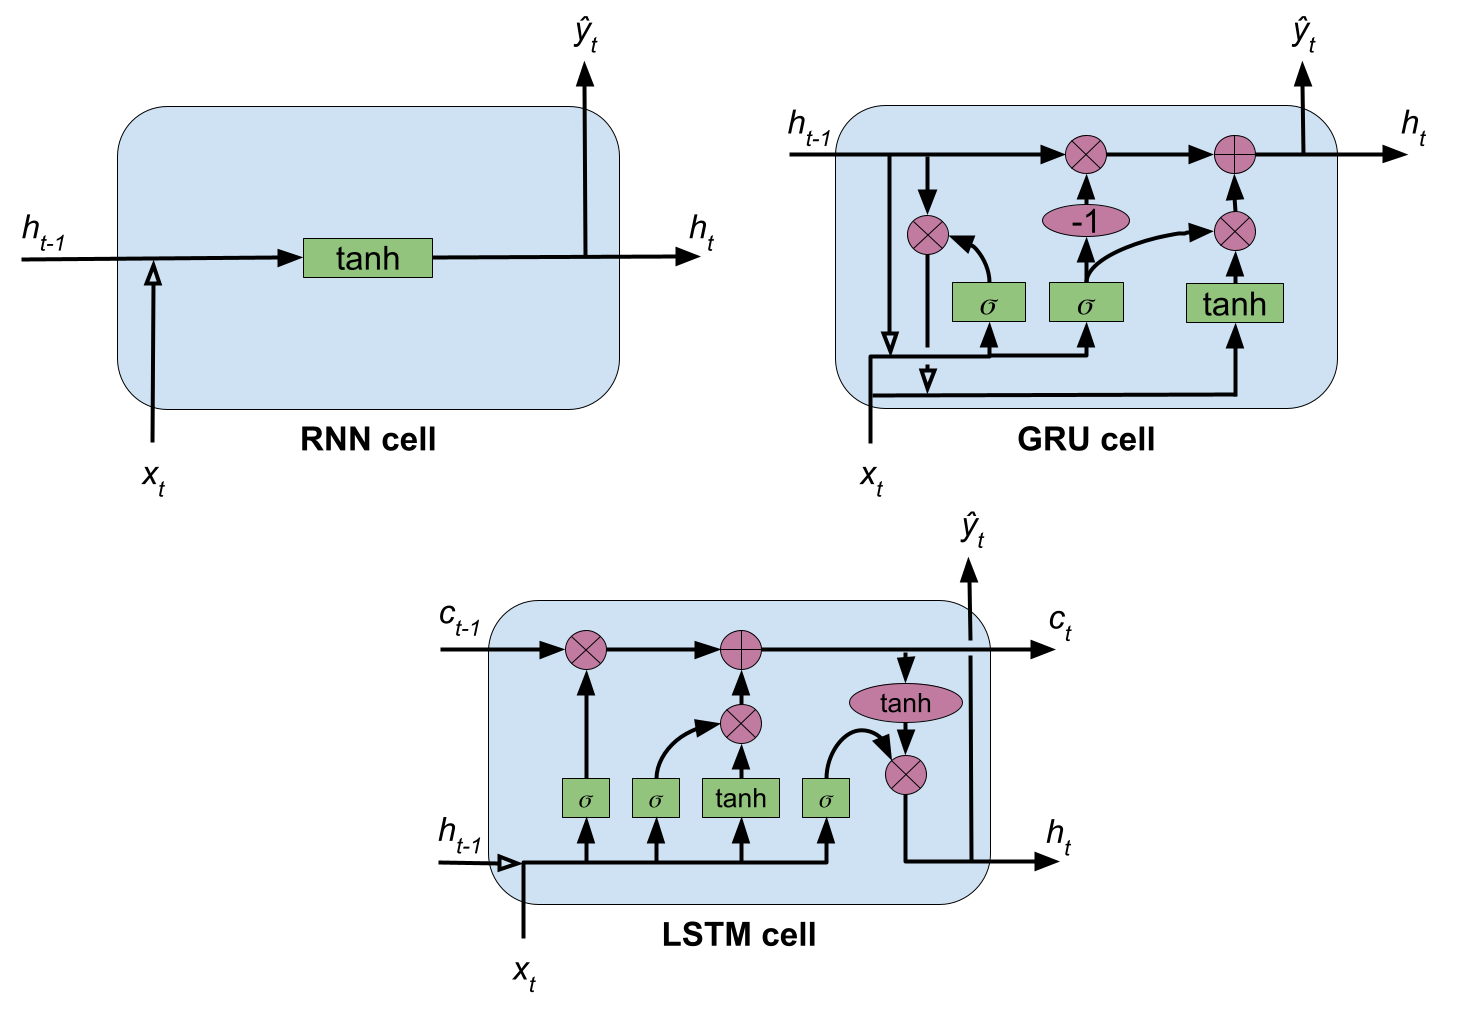
\includegraphics[width=0.8\linewidth]{figures/learning_quadrotor/cells.png}%
    \caption{Representation of a \myglsentry{rnn} cell (left), a \myglsentry{gru} cell (center), and a \myglsentry{lstm} cell (right).
    The three models (RNN, LSTM, and GRU) feature different update mechanisms (inside the blue box). They each take as input a hidden state $h$ (with LSTM also taking a cell state $c$) and a current state from the sequence $x$, and output the updated hidden state.
    }%
    \label{fig:rnns}%
\end{figure}

\section{Method} \label{sec:method}

This section presents a multi-task learning neural network based on a GRU architecture, which takes as input the desired states of the dynamic system and outputs the nominal control inputs $\u_n$, as well as the uncertainty tubes around the states $\Rq$ and the control inputs $\Ru$. 

The resulting predictor, denoted as $\boldsymbol{g}$, aims at bypasses the intrinsic structure of the original set of \myglsentry{odes} considered in this thesis. 
These dependencies arise from the structure of the equations: Equation~(\ref{eq:ctrl}) computes the control inputs, Equation~(\ref{eq:dyna}) updates the robot state, and Equation~(\ref{eq:dyna_sensi}) computes the sensitivity matrices before projecting them to derive the uncertainty tubes (see Equation~(\ref{eq:radius})). 
Note that each equation depends on the outputs of the preceding one within a single time step.

\subsection{Problem statement}

The goal is to train a neural network to approximate sensitivity-based uncertainty tubes, hence avoiding the computational cost of solving many \myglsentry{odes}. 
Moreover, the model aims at predicting the control inputs that the system will exert to successfully track a desired trajectory, in addition to the uncertainty tubes on these control inputs. 
Given a sequence of desired robot state vectors $\textbf{M} = \{\q_{d}^0, \q_{d}^1, ..., \q_{d}^n\}$ representing the desired robot motion (i.e. a desired trajectory to follow), the task at hand is to learn a function $\boldsymbol{g}$ that estimates the radii of uncertainty tubes for each state $\q_{d}^k$ as well as the robot control inputs at this state such that:
\begin{equation}\label{eq:prob_statement}
\{\Rq^{k}, \Ru^{k},\u^{k}\} = \boldsymbol{g}(\q_{d}^0, \q_{d}^1, ... \q_{d}^{k-1})
\end{equation}
Since evaluating the function $\boldsymbol{g}$ on $\q_{d}^k$ depends on all the previous states of the robot in $\textbf{M}$, recurrent neural network architectures are a good fit given their ability to encode and accumulate temporal information while keeping inference time low.

\subsection{Neural network architecture}\label{sec:architecture}

\begin{figure} [htp]
    \centering
    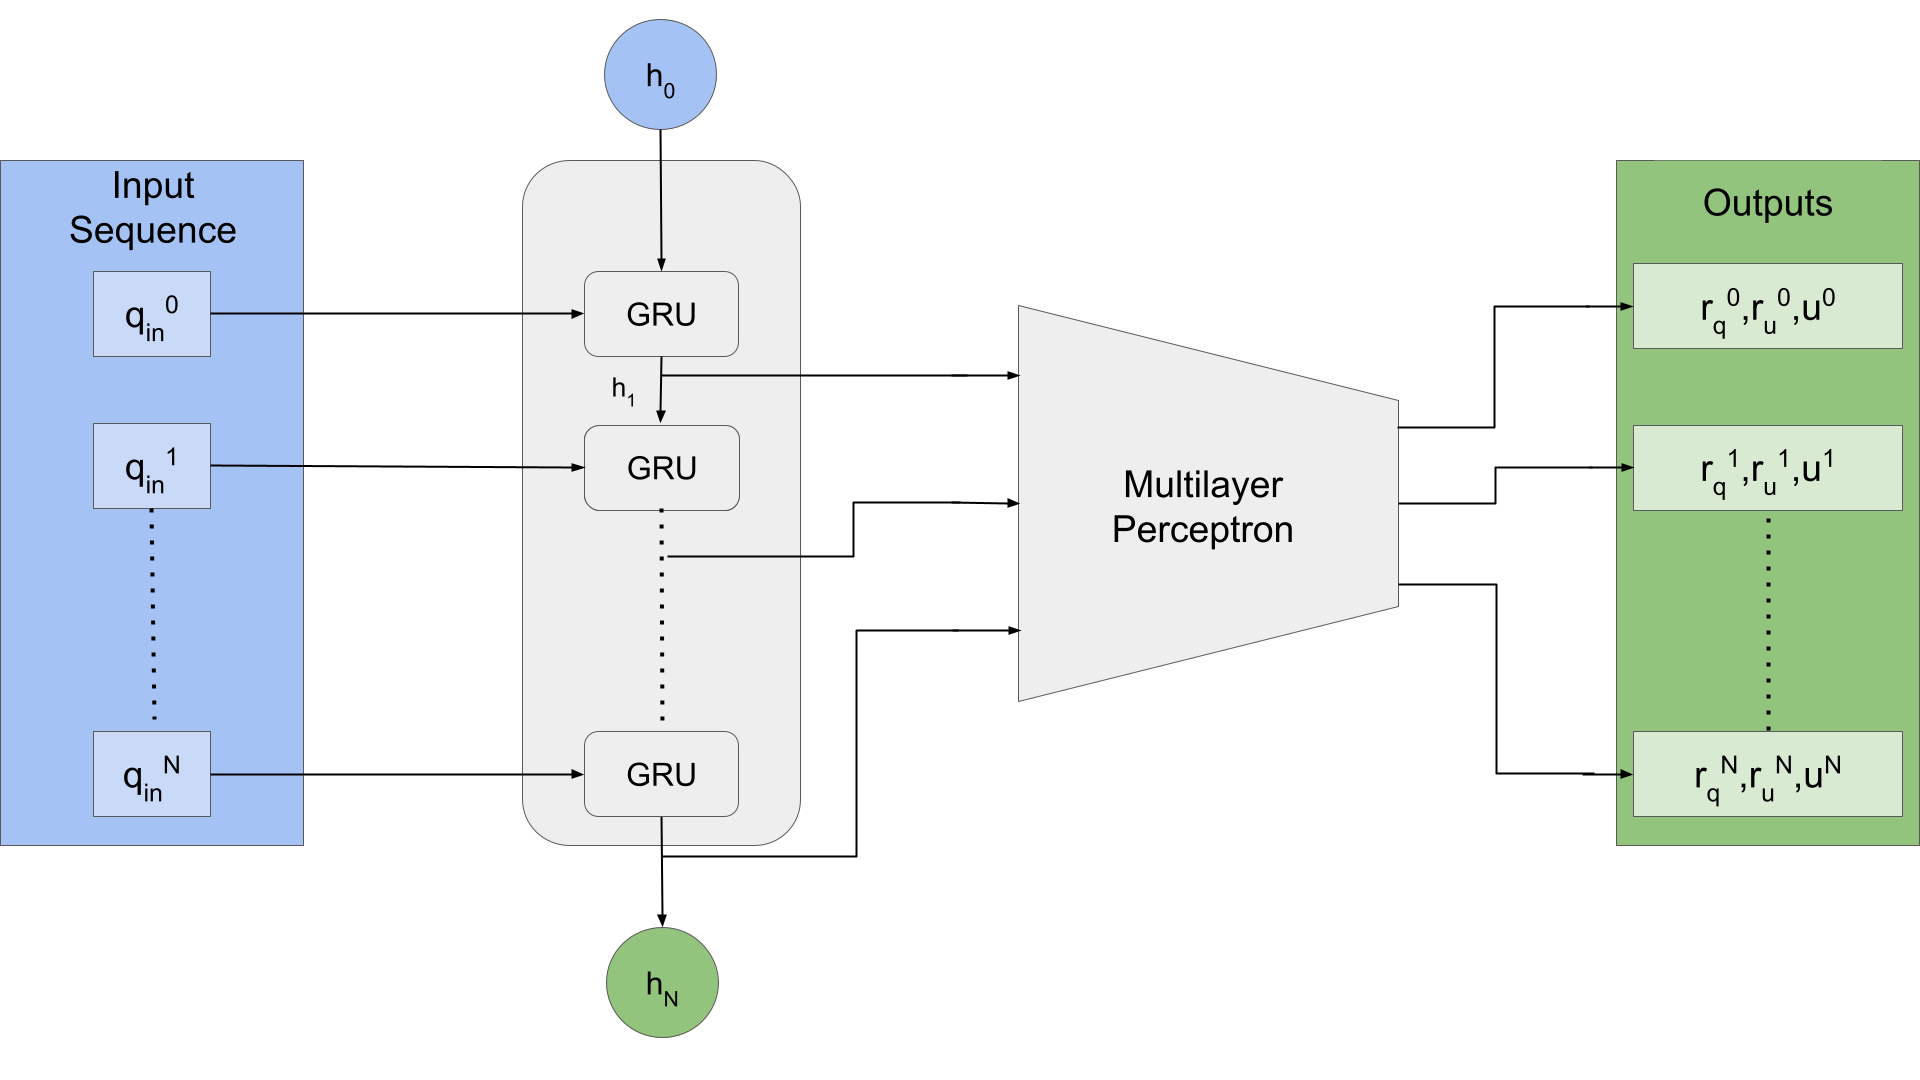
\includegraphics[width=0.8\linewidth]{figures/learning_quadrotor/SensiNN_GRU.png}%
    \caption{Representation of the proposed neural network architecture.
    }%
    \label{fig: NN}%
\end{figure}

A representation of the neural network architecture is presented in Figure~\ref{fig: NN}.
Blue blocks refer to the inputs of the model which are composed of an initial hidden state $\boldsymbol{h}_{0}$ and of a sequence of desired robot states evaluated along a desired trajectory denoted $\boldsymbol{\q_{in}^k}$, where $k$ refers to the $k$-th state of the desired trajectory. 

The outputs of the neural network correspond to the green blocks.
It is composed of the predicted uncertainty tubes radii along the state $\Rq$ and of the uncertainty tubes radii associated with the control inputs of the system $\Ru$.
Moreover, the control input values $\u$ are required for the motion planning algorithm to perform robust feasibility checks, and their computation depends on \myglsentry{odes} forward integration (as shown in Section~\ref{sec:tubes}). 
Since the proposed approach aims at eliminating the need for solving \myglsentry{odes}, the neural network is also trained to predict the control inputs.
However, note that the nominal states are intentionally not included in the learning process, as doing so would significantly increase the number of outputs and complicate the training process. 
Nevertheless, the control inputs are learned, as they enable efficient and fast filtering of infeasible trajectories in the motion planning context, as discussed in Chapter~\ref{chap:sampNN}.
Finally, $\boldsymbol{h}_{N}$ corresponds to the hidden state at the last point of our sequence (i.e., the last desired trajectory state).

At $k=0$, the first state in the input sequence $\boldsymbol{\q_{in}^0}$ and the initial hidden state $\boldsymbol{h}_0$ are given to a single-layer GRU block, which outputs an updated hidden state $\boldsymbol{h}_1$. 
The latter is then fed to a multi-layer perceptron (MLP), each layer followed by a ReLU activation function except the final one, to obtain the predicted control inputs $\u^0$, the state uncertainty tubes $\Rq^0$ as well as the control uncertainty tubes $\Ru^0$. 
The updated hidden state $\boldsymbol{h}_1$ is then given back to the GRU block along with the second element of the input sequence. 
This process is repeated for each element $\boldsymbol{\q_{in}^k}$ until all predictions are obtained.

The network is intended to be used in a sampling-based tree planner (see Chapter~\ref{chap:sampNN}), where local trajectories are concatenated to form a global one. 
Thus, since the hidden state encodes and accumulates temporal information about the input sequence, the final hidden state $\boldsymbol{h}_{N}$ of a local trajectory obtained after an iteration of a sampling-based tree planner can be saved and then given back as the initial hidden state $\boldsymbol{h}_{0}$ for future local trajectories considered during the next iterations. 
Therefore, in practice, this initial hidden state is generally not null.

\subsubsection{Differential drive robot}\label{sec:unic_nn_architecture}

As the proposed model aims to bypass solving the \myglsentry{odes}, which starts by computing the appropriate control inputs, a reasonable initial guess is to start the prediction using the same inputs as those used by the controller.
The \myglsentry{dfl} controller inputs consist of the desired robot position, linear velocities, and accelerations, as shown in Equation~\ref{eq:unic_control_law}. 
However, to ensure that the learned model is independent of the workspace boundaries used during planning (i.e., the robot's position limits) and since accelerations are not considered for this robot in this thesis, only the desired linear velocities are retained as input components for the network.
Therefore, the input to the neural network for the differential drive robot case is a vector $\boldsymbol{\q_{in}^k} = [\boldsymbol{v_d}]^T \in \mathbb{R}^2$, where $k$ refers to the $k$-th state of the desired trajectory.

The predicted outputs are composed of the predicted uncertainty tubes radii along the $\{x,y\}$-axis of the state $\Rq=$[$r_{x},\,r_{y}]^T \in \mathbb{R}^2$, and the uncertainty tubes radii associated with the control inputs of the system $\Ru = [r_{u1},\,r_{u2}]^T \in \mathbb{R}^2$.
The control input values predicted by the neural network are $\u = [u_1 ,\, u_2]^T \in \mathbb{R}^2$, which correspond to the right and left wheel speeds.

\subsubsection{Quadrotor}\label{sec:quad_nn_architecture}

In the quadrotor case, the controller inputs consist of the desired robot position, linear velocities, accelerations, yaw angle orientation, and yaw angular velocities, as shown in Equation~\ref{eq:desftau}. 
However, in order to make the learned model independent of workspace boundaries used during planning (i.e. robot position and orientation bounds) and initial robot orientations, only the desired linear velocities, accelerations, and yaw angular velocities ($\Dot{\Psi}_d$), are kept as the network input components.
Hence, the input to the neural network for the quadrotor case is a vector $\boldsymbol{\q_{in}^k} = [\boldsymbol{v_d} ,\, \boldsymbol{a_d} ,\, \Dot{\Psi}_d]^T \in \mathbb{R}^7$, where $k$ refers to the $k$-th state of the desired trajectory.

The predicted outputs for the quadrotor case, are composed of the predicted uncertainty tubes radii along the $\{x,y,z\}$-axis of the state $\Rq=$[$r_{x},\,r_{y},\,r_{z}]^T \in \mathbb{R}^3$, and the uncertainty tubes radii associated with the control inputs of the system $\Ru = [r_{u1},\,r_{u2},\,r_{u3},\,r_{u4}]^T \in \mathbb{R}^4$.
The control input values predicted by the neural network are $\u = [u_1 ,\, u_2 ,\, u_3 ,\, u_4]^T \in \mathbb{R}^4$, which correspond to the squared propeller speeds.

\subsection{Dataset}\label{sec:dataset_general}

\begin{figure} [htp]
    \centering
    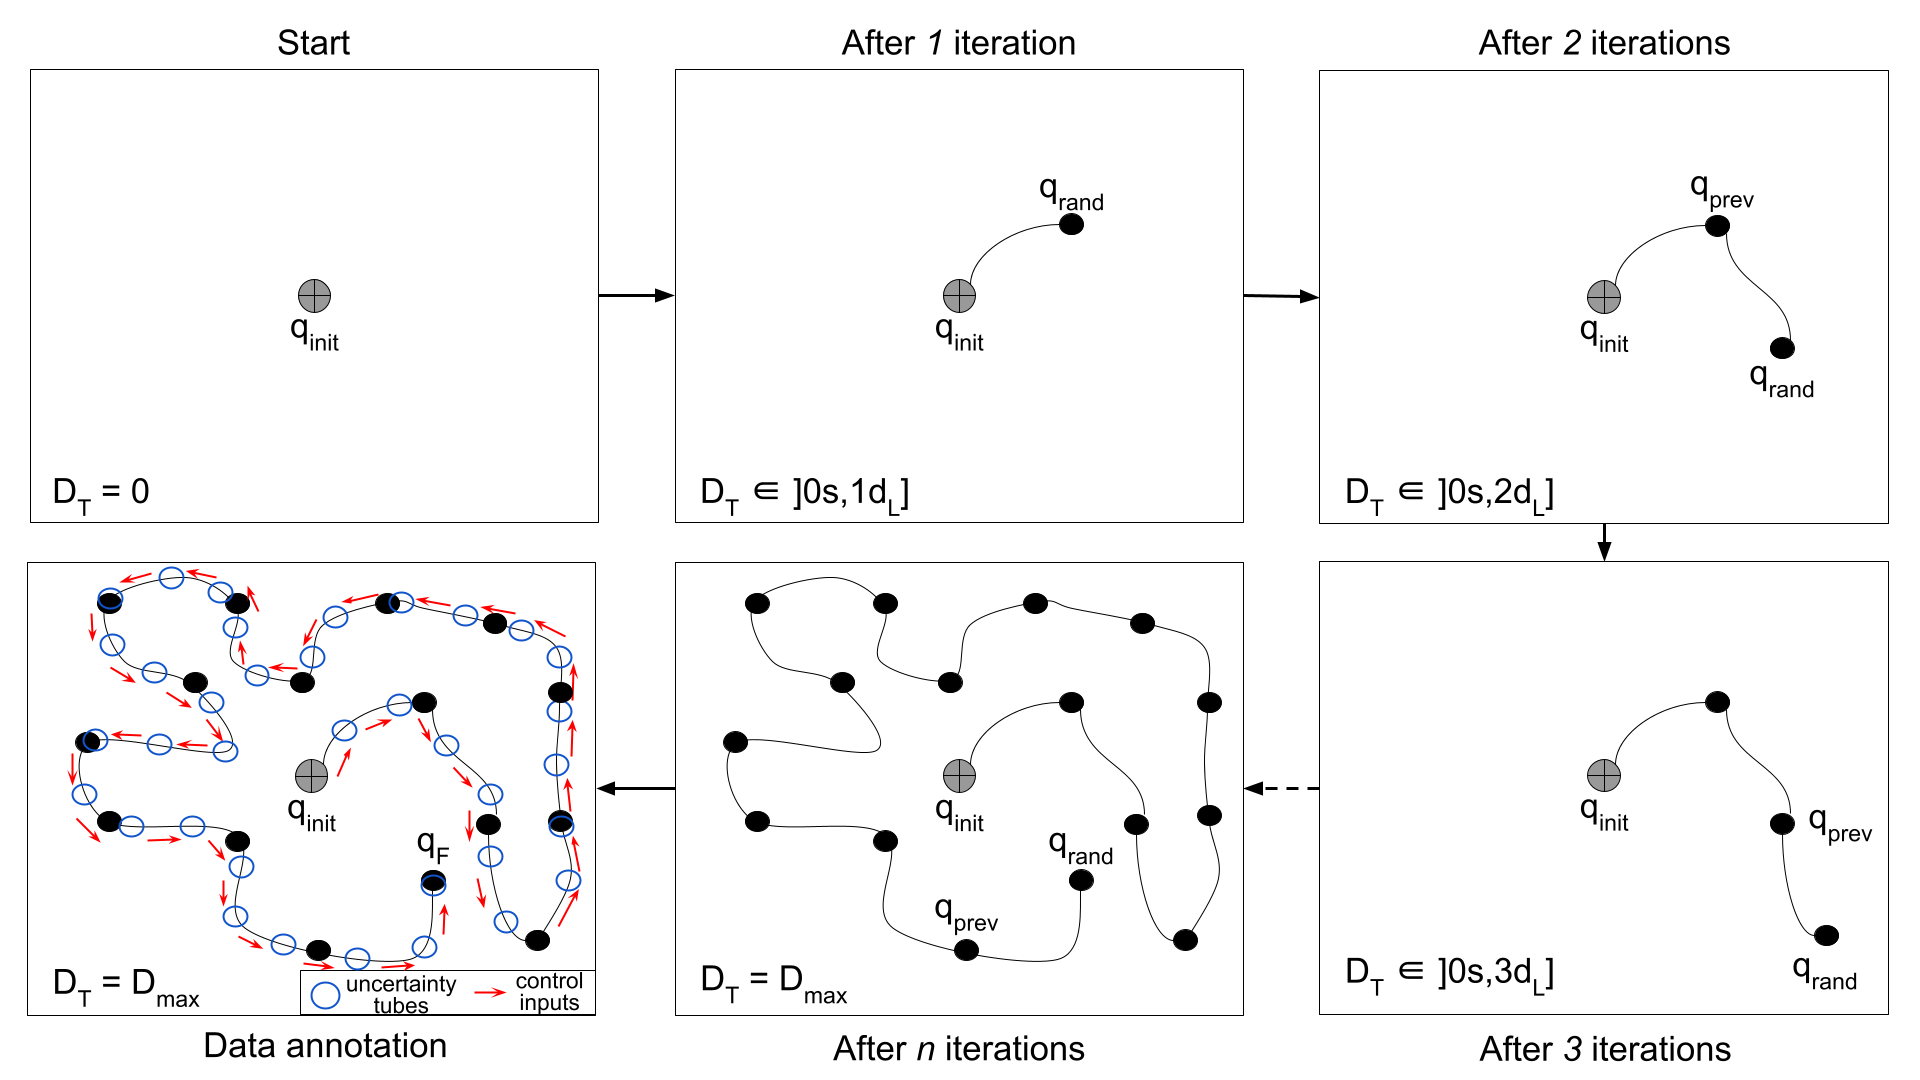
\includegraphics[width=0.9\linewidth]{figures/learning_quadrotor/dataset_generation.png}%
    \caption{Dataset generation process. 
    Starting from a stationary state $\q_{init}$, at each iteration a new state $\boldsymbol{q_{rand}}$ is randomly sampled and connected to the nearest one among the previous states $\boldsymbol{q_{prev}}$ until a total distance ($D_T$) equal to $D_{max}$ is reached.
    Data annotation is performed by simulating the tracking of the generated trajectory under nominal parameters.
    }%
    \label{fig: data_generation}%
\end{figure}

In order to train the proposed neural network, a dataset of trajectories computed in an obstacle-free environment is generated, as depicted in Figure~\ref{fig: data_generation}.
This ensures that the resulting learned model is totally independent of the environment and only depends on the system.
As a result, it is highly efficient when used in a sampling-based motion planning context, where the same robot model can be applied across different environments.

Each global trajectory starts from the same initial state ($\q_{init}$) initialized at zero velocities and accelerations.
Note that this initialization does not hurt the generalizability of the model to different initial conditions as every dynamic state can be connected to the null state by mean of a local planner.
Based on the same principle as a sampling-based planner, the global trajectory is made up of local sub-trajectories until a total distance $D_{max}$ (according to the state space metric) is reached.
Each local sub-trajectory is generated by uniformly sampling an arrival state ($\q_{rand}$) and connecting it to the nearest one among the previous sampled states ($\q_{prev}$) using an appropriate local planner, based on the robot being considered.
If the local trajectory (between $\boldsymbol{q_{rand}}$ and $\boldsymbol{q_{prev}}$) distance (according to the state space metric) is greater than a maximum local distance $d_l$, it is truncated to $d_l$. 
This maximum local distance refers to the planner maximum local distance (see Section~\ref{sec:samp_simu}).
Similarly, when the total distance exceeds $D_{max}$ after adding a new state, it is truncate at $D_{max}$.
This dataset generation process is similar to the construction of tree branches, with exported trajectories made of sub-trajectories to ensure the dataset accurately captures the behavior at the connections between tree nodes.

To generate the outputs, i.e. to annotate the data with uncertainty tubes and control inputs, the closed-loop dynamic and the sensitivity matrices are computed by simulating the tracking of the global trajectories using an integration time step $\Delta T$ which corresponds to the controller time step.
The data annotation was performed by computing and integrating the set of \myglsentry{odes} composed of Equation~(\ref{eq:dyna}), Equation~(\ref{eq:ctrl}), and Equation~(\ref{eq:dyna_sensi}) by mean of the Euler \myglsentry{odes} solver along a desired trajectory. 
Once $\bPi$ and $\bTheta$ had been computed, a simple projection was performed to recover the tubes thanks to Equation~(\ref{eq:radius}).
Note that the control inputs $\u$ are computed during the \myglsentry{odes} resolution.

Using this mechanism, a training set composed of 8.000 trajectories and a validation set composed of 2.000 trajectories were generated for both the quadrotor and the differential drive robots, making sure that every trajectory in the dataset is different.

\subsubsection{Differential Drive Robot}\label{sec:dataset_unic}

\begin{table}[htp]
    \centering
    \begin{tabular}{ | c | c || c |}
    \hline
      \textbf{Output}  & \textbf{Validation set}  & \textbf{Test set} \\ \hline
    $\Rq$ & $5.8e^{-2} \pm 2.2e^{-2}$ & $6.1e^{-2} \pm 2.3e^{-2}$ \\ \hline
    $\u$ & $15.1 \pm 1.3$ & $15.7 \pm 1.4$ \\ \hline
    $\Ru$ & $2.0e^{-1} \pm 7.8e^{-2}$ & $2.0e^{-1} \pm 8.1e^{-2}$ \\ \hline
\end{tabular}
\caption{
Mean and standard deviation of the output vector components norm after data annotation for the validation and test sets for the differential drive robot case.
$\Rq$ is expressed in \emph{m}, and $(\u, \Ru)$, are wheel angular velocities [(rad/s)].}
 \label{tab:datas_stats_unic}
\end{table}

The local planner used to generate the differential drive robot datasets is the Dubins method (see Section~\ref{sec:dubins}).
The trajectories in the dataset were generated with a maximum total distance $D_{max}$ of 15m, a maximum local distance of $d_l = 1m$, a velocity magnitude of $v_{magn} = 1 m.s^{-1}$, and an integration time step $\Delta T = 0.05s$. 

The robot model used for data annotation is the one described in Section~\ref{sec:unic_model}, with the following set of uncertain parameters $\p = [r, \, d]^T \in \mathbb{R}^{2}$.
The nominal values of the uncertain parameters used for the robot model are  $\p_n = [0.1m, \, 0.4m]^T$, with an associated uncertainty range of $\delta\p = [3\%, \, 3\%]^T$, representing the percentage deviation from their corresponding nominal values.
The controller gains are $\k_c = [1.5, \, 8.0, \, 0.2]^T$.

To demonstrate the reliability and generalizability of the learned model, a test set comprising 1.000 trajectories was generated using the same procedure, but with a velocity magnitude of $v_{magn} = 1.1 m.s^{-1}$ for the Dubins curve parametrization. 
Consequently, the test set includes trajectories with higher velocities than those in the validation set.

The mean and standard deviation values of the various components of the output vector for both the validation and test sets generated by this setup are presented in Table~\ref{tab:datas_stats_unic}. 
These values indicate a slight increase in the norms of all components due to the higher velocities.

\subsubsection{Quadrotor}\label{sec:dataset_quad}

\begin{figure} [htp]
    \centering
    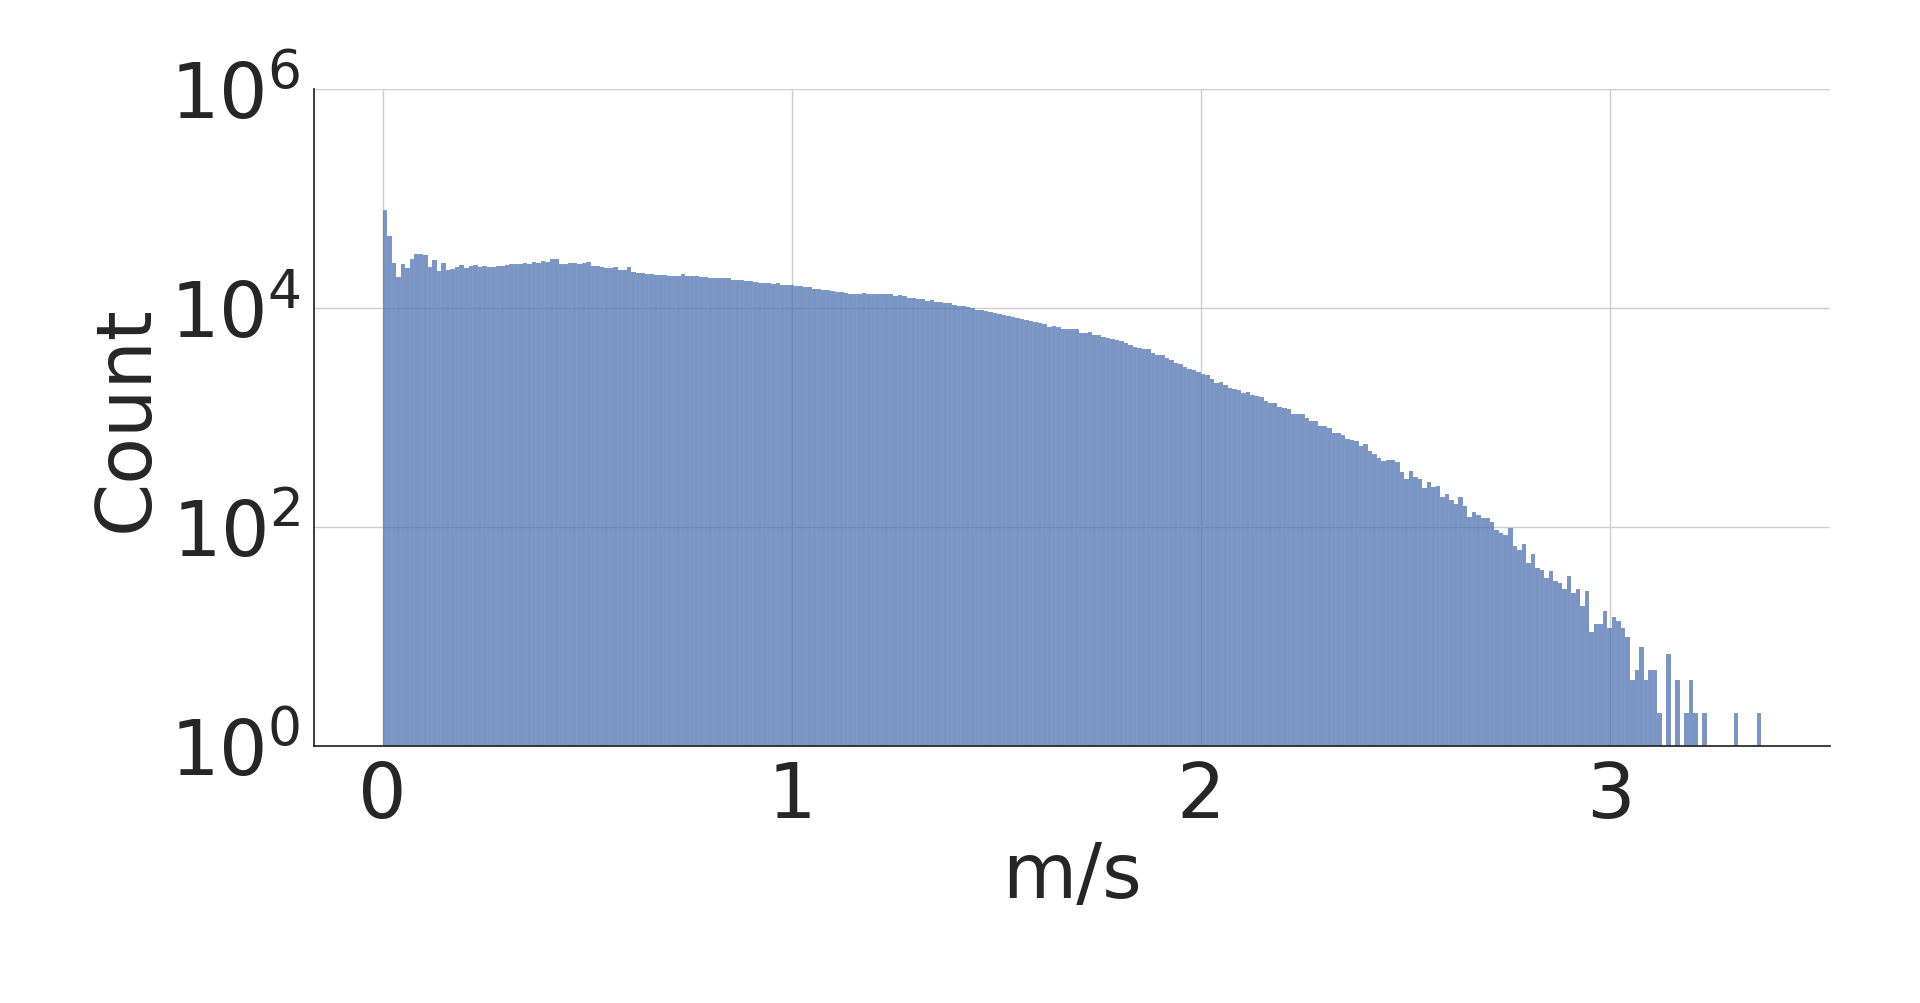
\includegraphics[width=0.49\linewidth]{figures/learning_quadrotor/vnorm_val2.png}
    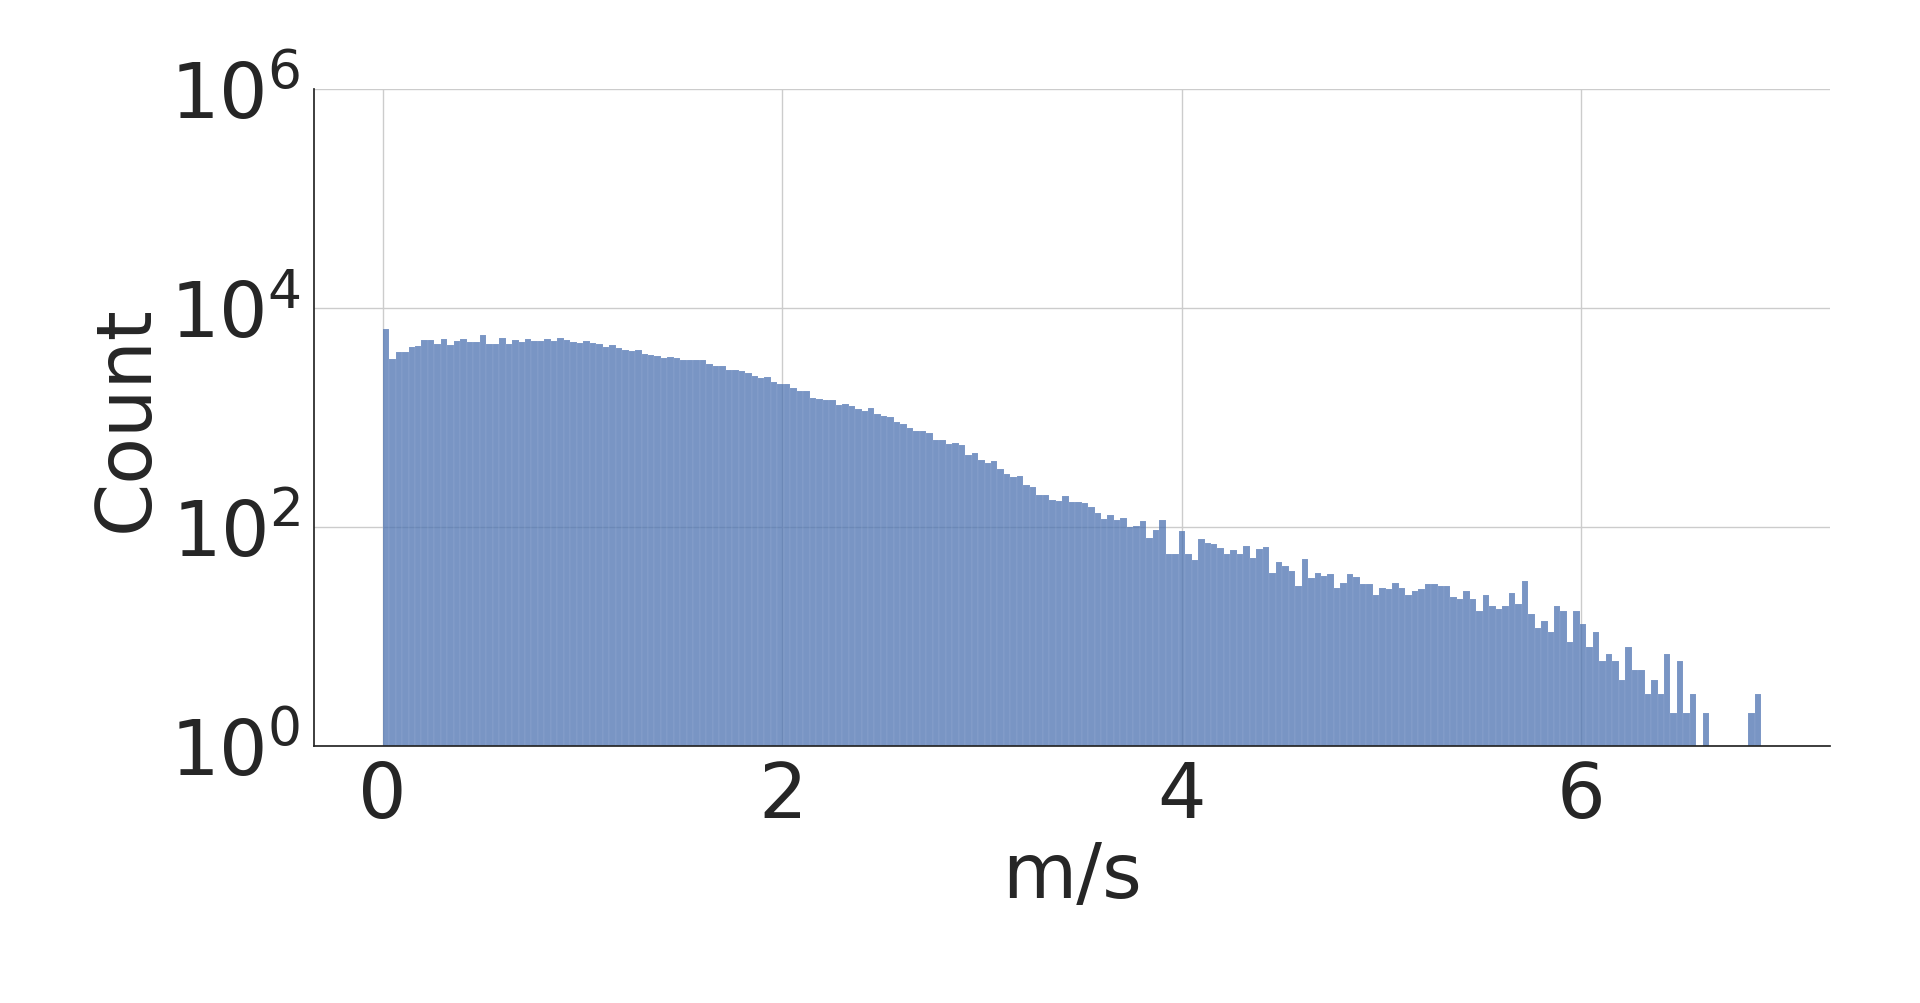
\includegraphics[width=0.49\linewidth]{figures/learning_quadrotor/vnorm_test.png}
    \caption{Velocity norm distribution in the training (left) and test sets (right) for the quadrotor.}%
    \label{fig: valvstest}%
\end{figure}

\begin{table}[htp]
    \centering
    \begin{tabular}{ | c | c || c |}
    \hline
      \textbf{Output}  & \textbf{Validation set}  & \textbf{Test set} \\ \hline
    $\Rq$ & $1.0e^{-1} \pm 2.0e^{-2}$ & $1.1e^{-1} \pm 2.1e^{-2}$ \\ \hline
    $\u$ & $12469.3 \pm 861.6$ & $12476.8 \pm 1016.5$ \\ \hline
    $\Ru$ & $7782.6 \pm 3172.3$ & $7828.6 \pm 2845.7$ \\ \hline
\end{tabular}
\caption{
Mean and standard deviation of the output vector components norm after data annotation for the validation and test sets for the quadrotor case.
$\Rq$ is expressed in \emph{m}, and $(\u, \Ru)$, are squared propeller angular velocities [(rad/s)²].}
 \label{tab:datas_stats}
\end{table}

The local planner used to generate the quadrotor datasets is the kinosplines method described in Section~\ref{sec:kinosplines}, that enforced the following kinodynamic constraints on the generated splines $[v_{max}, a_{max}, j_{max}, s_{max}] = [5.0 \, m.s^{-1}, \allowbreak 1.5 \, m.s^{-2}, \allowbreak 15.0 \, m.s^{-3}, \allowbreak 30.0 \, m.s^{-4}]$. 
The trajectories of the dataset were generated considering a total distance $D_{max}$ of 15s, a maximum local distance of $d_l = 1s$ and an integration time step $\Delta T = 0.05s$. 

The quadrotor model used for data annotation is the one described in Section~\ref{sec:quad_model}, with the following set of uncertain parameters $\p$ = $[m, \, \allowbreak x_{cx}, \, \allowbreak x_{cy}, \, \allowbreak J_{x}, \, \allowbreak J_{y}, \,\allowbreak J_{z}]^T \in \mathbb{R}^{6}$, with $m$ the quadrotor mass, $x_{cx,y}$ a shift of the system center of mass along the \{x,y\}-axis, and $J_{x,y,z}$ the main inertia coefficients.
The nominal values of the uncertain parameters used for the robot model are $\p_{n}$ = $[1.113, \allowbreak0.0, \allowbreak0.0, \allowbreak0.015, \allowbreak0.015, \allowbreak0.007]^T$ and their associated uncertainty range used for the tubes computation are $\delta\p = [7\%, \allowbreak3cm, \allowbreak3cm, \allowbreak10\%, \allowbreak10\%, \allowbreak10\%]^T$, which represents the variation of the parameters w.r.t. their associated nominal value.
This choice of uncertain parameters is discussed in relation to the experimental validation presented in Chapter~\ref{chap:sampNN}.
The controller gains are $\boldsymbol{k}_{x} = [20.0, \, 20.0, \, 25.0]^T$, $\boldsymbol{k}_{v}= [9.0, \, 9.0, \, 12.0]^T$, $\boldsymbol{k}_{R}=[4.6, \, 4.6, \, 0.8]^T$, and $\boldsymbol{k}_{\omega}=[0.5, \, 0.5, \, 0.08]^T$.

In order to show the reliability and generalizability of the learned model, a test set composed of 1.000 trajectories was generated in the same way, but considering a maximum local duration $d_l = 2s$.
As a result, trajectories with higher velocities are encountered in the test set compared to the validation set, as depicted in Figure~\ref{fig: valvstest} where velocity norms can reach up to 7 m.s$^{-1}$ in the test set, compared with only 3 m.s$^{-1}$ in the validation set.
Note that the velocity norms exceed the velocity limit $v_{max}$, this is expected since this limit applies to the components of the velocity vector rather than the norm.

The mean and standard deviation values of the various components of the output vector for the validation and test sets generated by this setup are provided in Table~\ref{tab:datas_stats}.

\section{Evaluation}\label{sec:nn_eval}

In order to demonstrate the necessity of using a recurrent neural network due to the temporal dependencies of the predictions, a simple \textbf{MLP} baseline is implemented by substituting the recurrent layer with a single-layer linear encoder which takes as input a single element in the sequence and outputs its corresponding predictions.
Also, in order to justify the choice of a \textbf{GRU} architecture, the proposed model is compared to two other versions which replace the GRU block by a basic RNN \cite{cRNN} and an LSTM \cite{cLSTM} block respectively.

Finally, in order to measure the computational cost gain achieved by the proposed method and compare the inference time of the neural network to traditional methods, two known \myglsentry{odes} integrators are implemented for computing uncertainty tubes.
The first is \textbf{dopri5}, which leverages the Runge Kutta-4 algorithm to numerically approximate the solutions to \myglsentry{odes}. 
The second is the \textbf{Euler} method, which is known to be faster but yields less accurate results.

\subsection{Metrics}\label{sec:metric}

The performance of the model is evaluated using the Mean Absolute Error (MAE) over the different outputs. 
Rather than comparing the results on each sub-component of the input (e.g $\{x, y, z\}$ for $\Rq$ in the quadrotor case), they are combined into a single metric in order to obtain simpler and more general comparisons, as follows:
\begin{itemize}
    \item $\mathbf{MAE_{\Rq}}$ : represents the mean absolute error on the norm of $\Rq$. 
    For a given datapoint, given the ground truth and predicted state uncertainty tubes $\Rq$ and $\mathbf{\hat{r}_q}$, their respective norms $\|\Rq\|$ and $\|\mathbf{\hat{r}_q}\|$, are computed. 
    The mean absolute error, $\mathbf{MAE_{\Rq}}$, is then defined as:
    \begin{equation}\label{eq:MAE rq}
        \mathbf{MAE_{\Rq}} = MAE(\|\Rq\|, \|\mathbf{\hat{r}_q}\|)
    \end{equation}
    This metric is expressed in meters (m).
    \item $\mathbf{MAE_{u}}$ : represents the mean absolute error on the norm of $\u$. 
    The norms of the ground truth and predicted control inputs, $|\u|$ and $|\hat{\u}|$, are computed. 
    The mean absolute error, $\mathbf{MAE_{u}}$, is then calculated as the mean absolute error between these two norms. 
    It is expressed in [(rad/s)²] for the quadrotor case, and in [(rad/s)] for the differential drive robot one.
    \item $\mathbf{MAE_{\Ru}}$ : represents the mean absolute error on the norm of $\Ru$. 
    As for the two previous metrics, $\mathbf{MAE_{\Ru}}$ is defined as the mean absolute error between the norms $\|\Ru\|$ and $\|\mathbf{\hat{r}_u}\|$. 
    This metric is expressed in [(rad/s)²] for the quadrotor case, and in [(rad/s)] for the differential drive robot one.
\end{itemize}

These metrics are averaged over all elements of a sequence, then averaged over all sequences in the validation and test sets. 
In addition, the inference time is also used as metric in order to evaluate the computational cost of the method compared to the defined baselines, as well as traditional uncertainty tubes computation methods involving an ODE solver. 
Time is denoted $T_{solver/NN}$ according to the model or solver used.

\subsection{Training}

This subsection outlines the training procedures and specifies the neural network parameters used.

\subsubsection{Differential drive robot}

Before training the neural network, the input features of the dataset (train, val, and test) were min-max scaled according to the velocity magnitude value used when generating the dataset (see Section~\ref{sec:dataset_unic}) as it is guaranteed that the velocities components generated cannot exceed this value, ensuring that all velocity values are in the interval $[-v_{magn}, v_{magn}]$.  
The annotations were also normalized using a standard scaling based on the mean and standard deviation values of the training set annotations.

Finally, after data normalization, the neural networks were trained for 100 epochs using the Adam optimizer \cite{kingma2014adam} with an appropriate learning rate mentioned below and a batch size of 128. 
The \textbf{RNN},\textbf{LSTM} and \textbf{GRU} models were trained with a hidden state size of 128, a \textbf{MLP} composed of 3 linear layers, and a learning rate of $1e^{-3}$ for the \textbf{RNN}, the \textbf{LSTM} and \textbf{GRU} models.
Note that an LSTM layer is composed of a hidden state and a cell state (contrarily to GRUs and RNNs which have a hidden state only), so the real LSTM latent state size is 2$\times$128.
All used hyper-parameters were validated using a grid search.
They were trained using the MSE (Mean Squared Error) loss function and evaluated continuously on the validation set. 
The model weights achieving the best performance on the validation set were saved and used during the experiments.
The resulting learning curves can be found in appendix~\ref{chap:appendixB}.

\subsubsection{Quadrotor}\label{sec:train_quad}

Before training the neural network, the input features of the dataset (train, val, and test) were min-max scaled according to the maximum velocity and acceleration values used to generate the kinosplines (see Section~\ref{sec:dataset_quad}) as it is guaranteed that the velocities and accelerations generated cannot exceed these values. 
This ensures that all velocity values are in the interval $[-v_{max}, v_{max}]$, while all the acceleration values are in $[-a_{max}, a_{max}]$. 
The annotations were also normalized using a standard scaling based on the mean and standard deviation values of the training set annotations.

Finally, after data normalization, the neural networks were trained for 200 epochs using the Adam optimizer \cite{kingma2014adam} with an appropriate learning rate mentioned below and a batch size of 128. 
The \textbf{RNN},\textbf{LSTM} and \textbf{GRU} models were trained with a hidden state size of 512, a \textbf{MLP} composed of 3 linear layers, and a learning rate of $1e^{-4}$ for the \textbf{RNN} case against $1e^{-3}$ for both the \textbf{LSTM} and \textbf{GRU} models.
Note that an LSTM layer is composed of a hidden state and a cell state (contrarily to GRUs and RNNs which have a hidden state only), so the real LSTM latent state size is 2$\times$512.
All used hyper-parameters were validated using a grid search.
They were trained using the MSE (Mean Squared Error) loss function and evaluated continuously on the validation set. 
The model weights achieving the best performance on the validation set were saved and used during the experiments.
The resulting learning curves can be found in appendix~\ref{chap:appendixB}.

\subsection{Implementation details}

The ODEs were implemented using the JiTCODE \cite{cJit} module which converts the equations to be integrated into C-compiled code.
The \textbf{Euler} method or the \textbf{dopri5} integrator were then used to solve each ODE and take advantage of this compiled function.
Note that the \textbf{Euler} method is the one used to solve the \myglsentry{odes} during planning (see Chapter~\ref{chap:samp} and Chapter~\ref{chap:sampNN}).
Additionally, the \textbf{dopri5} integrator is also considered as a baseline for comparison, as it is a widely used implementation of the Runge-Kutta 4 method.

All the neural networks were implemented using the PyTorch library~\cite{cPytorch} and the lightning module.

All following results were obtained on an Intel i9 CPU@2.6GHz processor with one RTX A3000 GPU. 

\section{Simulation results}\label{sec:nn_results}

\subsection{Differential Drive Robot}\label{sec:nn_results_unic}

\subsubsection{Model comparison}\label{sec:nn_comparaison_unic}

Table~\ref{tab:NN_results_table_Q_unic} reports the MAE for the different output vector components on the validation and test sets. 
Firstly, one can note how the simple \textbf{MLP} model provides poor prediction accuracy across all components in both the validation and test sets.
This suggests that the \textbf{MLP} struggles to capture the strong temporal dependencies between inputs and outputs.
Consequently, the \textbf{MLP} shows the highest deviation from the ground truth values, as reported in Table~\ref{tab:datas_stats}, with deviations reaching up to 30\% for the $\Rq$ component in the validation set, and 32\% for the $\Ru$ component in the test set.

As for recurrent networks, the \textbf{RNN} demonstrates the poorest performance, with errors reaching up to 7\% on the validation set and 11\% on the $\Ru$ components of the test set.
The \textbf{GRU} and \textbf{LSTM} models exhibit comparable accuracy overall. 
However, the \textbf{GRU} slightly outperforms on the validation set, achieving only a 1\% deviation on both the $\Rq$ and $\Ru$ components, compared to the \textbf{LSTM}, which shows a 2\% deviation on $\Ru$.
While the \textbf{LSTM} generalizes better on $\Ru$ according to the results over the test set, the \textbf{GRU} achieves superior generalization on $\Rq$ and $\u$, making it the most robust model overall.
It is worth noting that the deviations observed on the test set are a bit high, reaching up to 6\% for the \textbf{GRU}. 
This indicates a slight overfitting of the model to the validation set.

Nevertheless, in a sampling-based context, the model accuracy alone is not sufficient as a performance metric.
As discussed in Section~\ref{sec:metric}, it is also essential to compare the inference time of the various models with the time required to integrate the \myglsentry{odes} using standard methods.
Table~\ref{tab:timepred_unic} shows the results obtained on trajectories of several hundred states. 
Note that with the current system, the number of ordinary equations solved for each element in the sequence (i.e. trajectory state) is equal to 16.
The results indicate that the average prediction gain time for neural networks is approximately of an order of magnitude compared to the \textbf{Euler} and \textbf{dopri5} methods. 
Additionally, note that even if the inference time appears to scale linearly with the number of time steps to be integrated, the time savings become increasingly significant with the number of states. 
Specifically, the \textbf{GRU} achieves a speedup of 15 times compared to \textbf{Euler} for 100 states, and this advantage grows to 35 times for 300 states.
This result suggests that the intrinsic structure of the original \myglsentry{odes}, as discussed in Section~\ref{sec:method}, has been reformulated into a simplified representation.

In conclusion, the \textbf{GRU} emerges as the most suitable model for sampling-based applications, offering the best balance between accuracy and inference time. 
While the \textbf{RNN} is the fastest, its accuracy is the lowest among the three recurrent architectures. 
On the other hand, the \textbf{LSTM} achieves accuracy comparable to the \textbf{GRU} but is slower in terms of inference speed.

\begin{table}[t]
\centering
\begin{tabular}{ | c | c  c  c | }
\hline
    \multirow{2}{*}{\textbf{Method}} & \multicolumn{3}{c|}{\textbf{Validation set}} \\ \cline{2-4}
    & \textbf{MAE$_{\Rq}$} $(m)$  & \textbf{MAE$_{\u}$} $[(rad/s)^2]$ & \textbf{MAE$_{\Ru}$} $[(rad/s)^2]$ \\ \hline
{\textbf{MLP}} & $1.8e^{-2}$ & $8.1e^{-1}$ & $6.2e^{-2}$ \\ 
{\textbf{RNN}} & $3.8e^{-3}$ & $1.1e^{-1}$ & $1.3e^{-2}$ \\ 
{\textbf{LSTM}} & $9.5e^{-4}$ & $7.2e^{-2}$ & $4.2e^{-3}$ \\ 
{\textbf{GRU}} & $\boldsymbol{6.9e^{-4}}$ & $\boldsymbol{4.4e^{-2}}$ & $\boldsymbol{3.3e^{-3}}$ \\ 
\hline
    & \multicolumn{3}{c|}{\textbf{Test set}}\\ \cline{2-4}
    & \textbf{MAE$_{\Rq}$} $(m)$  & \textbf{MAE$_{\u}$} $[(rad/s)^2]$ & \textbf{MAE$_{\Ru}$} $[(rad/s)^2]$ \\ \hline
{\textbf{MLP}} & $1.9e^{-2}$ & $1.4$ & $6.5e^{-2}$ \\ 
{\textbf{RNN}} &  $5.9e^{-3}$ & $6.1e^{-1}$ & $2.3e^{-2}$ \\ 
{\textbf{LSTM}} & $4.3e^{-3}$ & $5.6e^{-1}$ & $\boldsymbol{9.4e^{-3}}$ \\ 
{\textbf{GRU}} & $\boldsymbol{3.3e^{-3}}$ & $5\boldsymbol{.0e^{-1}}$ & $1.4e^{-2}$ \\ 
\hline
    
\end{tabular}
\caption{
MAE on the $\boldsymbol{r_q}$, $\boldsymbol{u}$ and $\boldsymbol{r_u}$ components of the output vector computed on the validation and test sets for a trained RNN, GRU, and LSTM model, for the differential drive robot.}
    \label{tab:NN_results_table_Q_unic}
\end{table}

\begin{table}[t]
\centering
\begin{tabular}{ | c | c  c  c | }
\hline
    \textbf{Time (ms)} & 100 states  & 200 states & 300 states \\ \hline
    $T_{euler}$ & $63.9 \pm 18.3$ & $136.7 \pm 29.9$ & $260.5 \pm 38.0$ \\ 
$T_{dopri5}$ & $251.7 \pm 17.3$ & $537.2 \pm 29.8$ & $755.6 \pm 34.5$ \\ 
$T_{RNN}$ & $\boldsymbol{0.9} \pm 0.3$ & $\boldsymbol{1.8} \pm 0.3$ & $\boldsymbol{2.2} \pm 0.5$ \\ 
$T_{LSTM}$ & $2.5 \pm 0.3$ & $4.8 \pm 0.3$ & $7.7 \pm 0.8$ \\ 
$T_{GRU}$(ours) & $2.1 \pm 0.2$ & $4.3 \pm 0.3$ & $5.8 \pm 0.4$  \\ \hline
\end{tabular}
\caption{
Average prediction time (ms) over 100 predictions on trajectories composed of 100 states, 200 states and 300 states, for an \textbf{RNN}, \textbf{GRU}, \textbf{LSTM}, the \textbf{Euler} integrator, and the \textbf{dopri5} integrator, for the differential drive robot.}
    \label{tab:timepred_unic}
\end{table}

\subsubsection{Qualitative results}

\begin{figure}[htp]
    \centering
    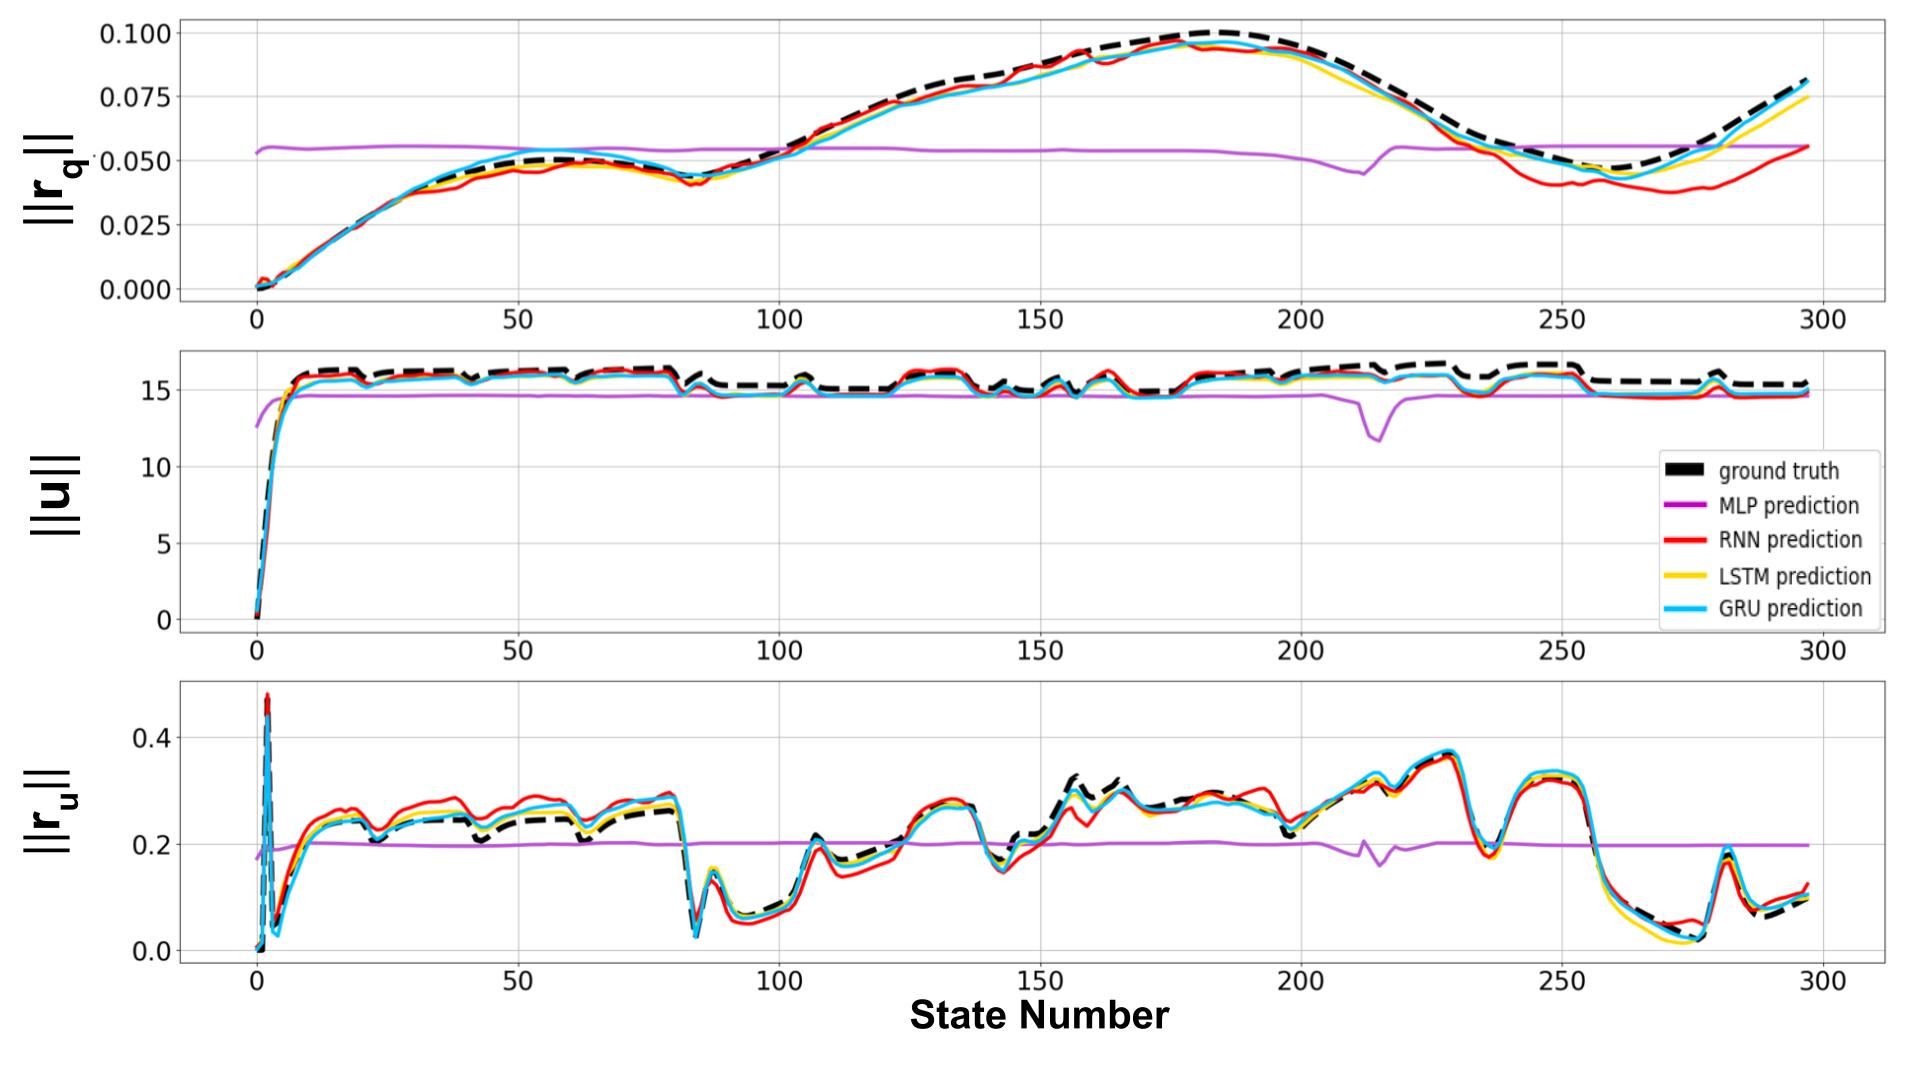
\includegraphics[width=0.99\linewidth]{figures/learning_unic/all_models_labeled.jpg} 
    \caption{Comparison of predictions obtained using the different recurrent neural network architectures as well as the \textbf{MLP} on a 300-state trajectory of the test set for the differential drive robot case. 
    $||\Rq||, ||\u||$ and $||\Ru||$ refer to the norm of their respective vector. 
    True values are displayed in black, \textbf{GRU} predictions in blue, \textbf{MLP} predictions in purple, \textbf{LSTM} outputs in yellow, and basic \textbf{RNN} predictions are in red.}
    \label{fig:all_models_pred_val_unic}
\end{figure}

\begin{figure}[htp]
    \centering
    \begin{minipage}{0.49\linewidth}
        \centering
        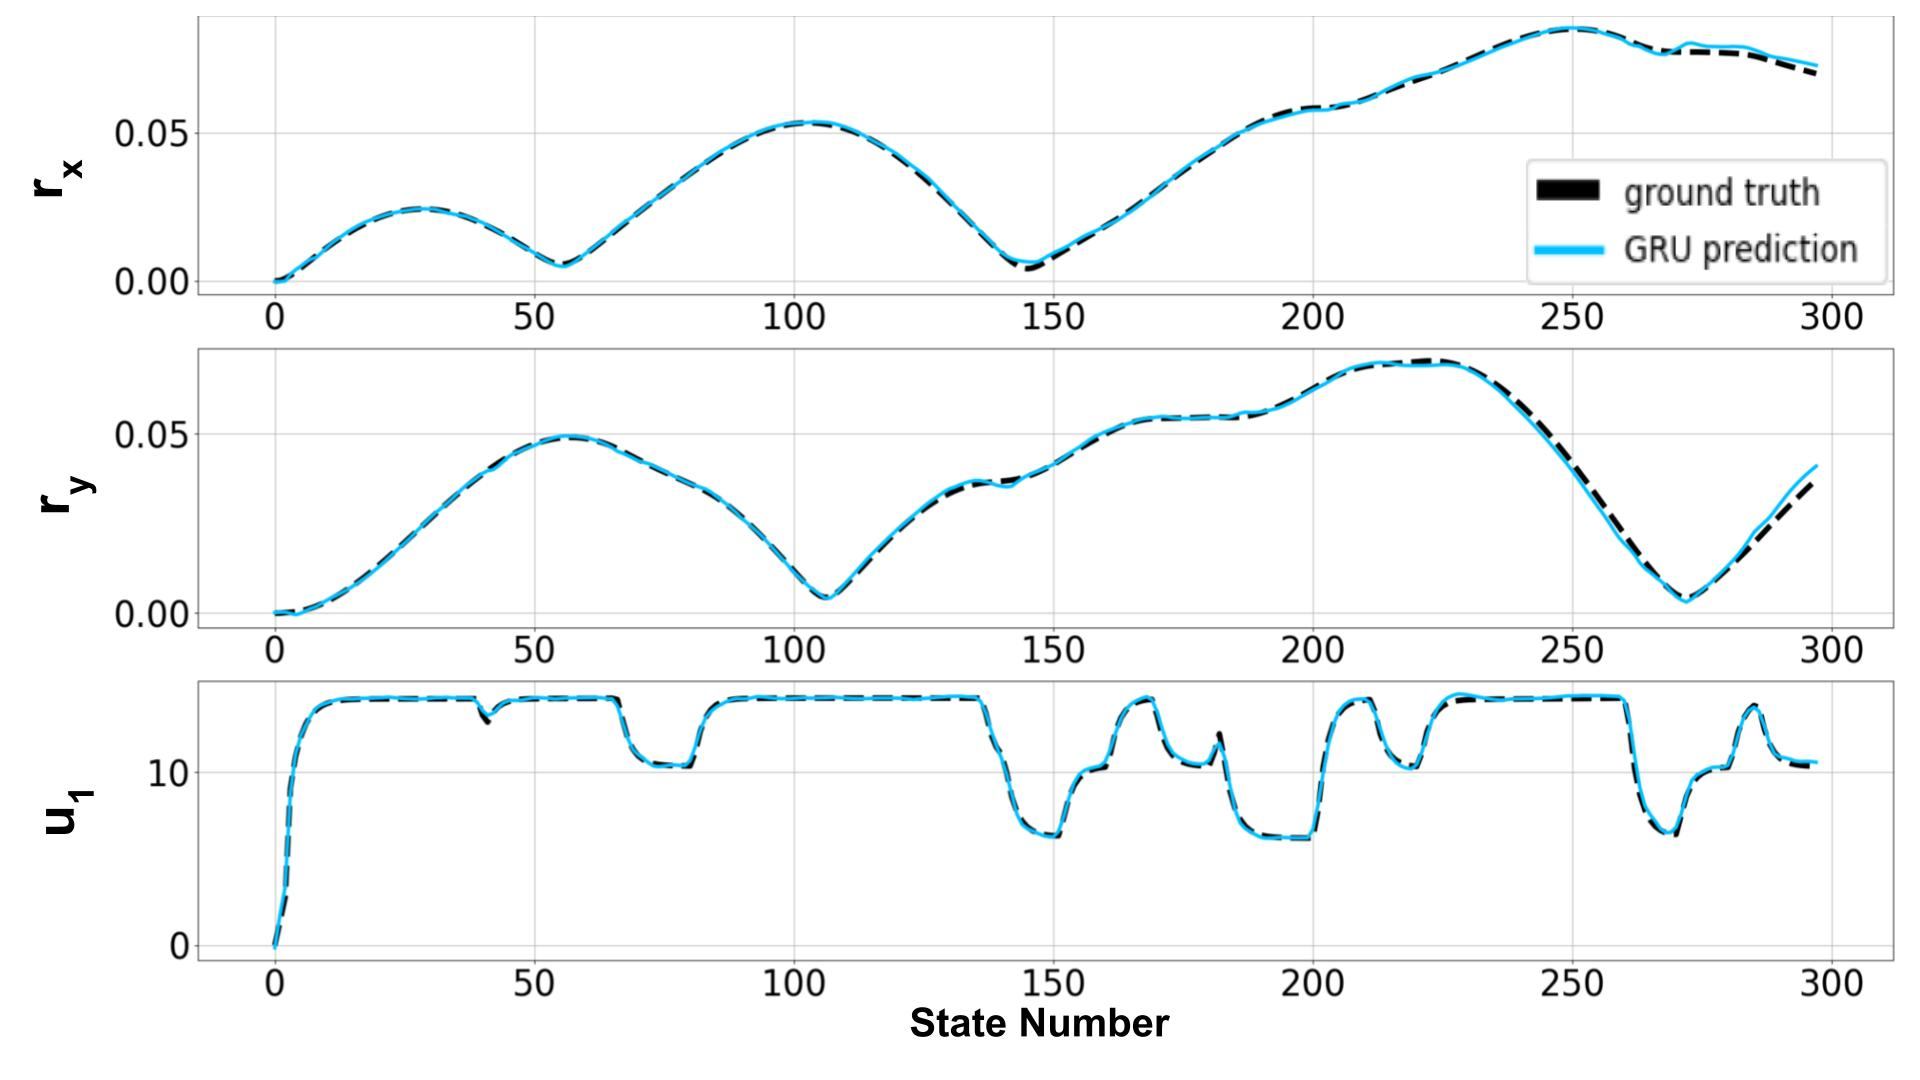
\includegraphics[width=\linewidth]{figures/learning_unic/pred_val_1_labeled.jpg}
    \end{minipage}
    \begin{minipage}{0.49\linewidth}
        \centering
        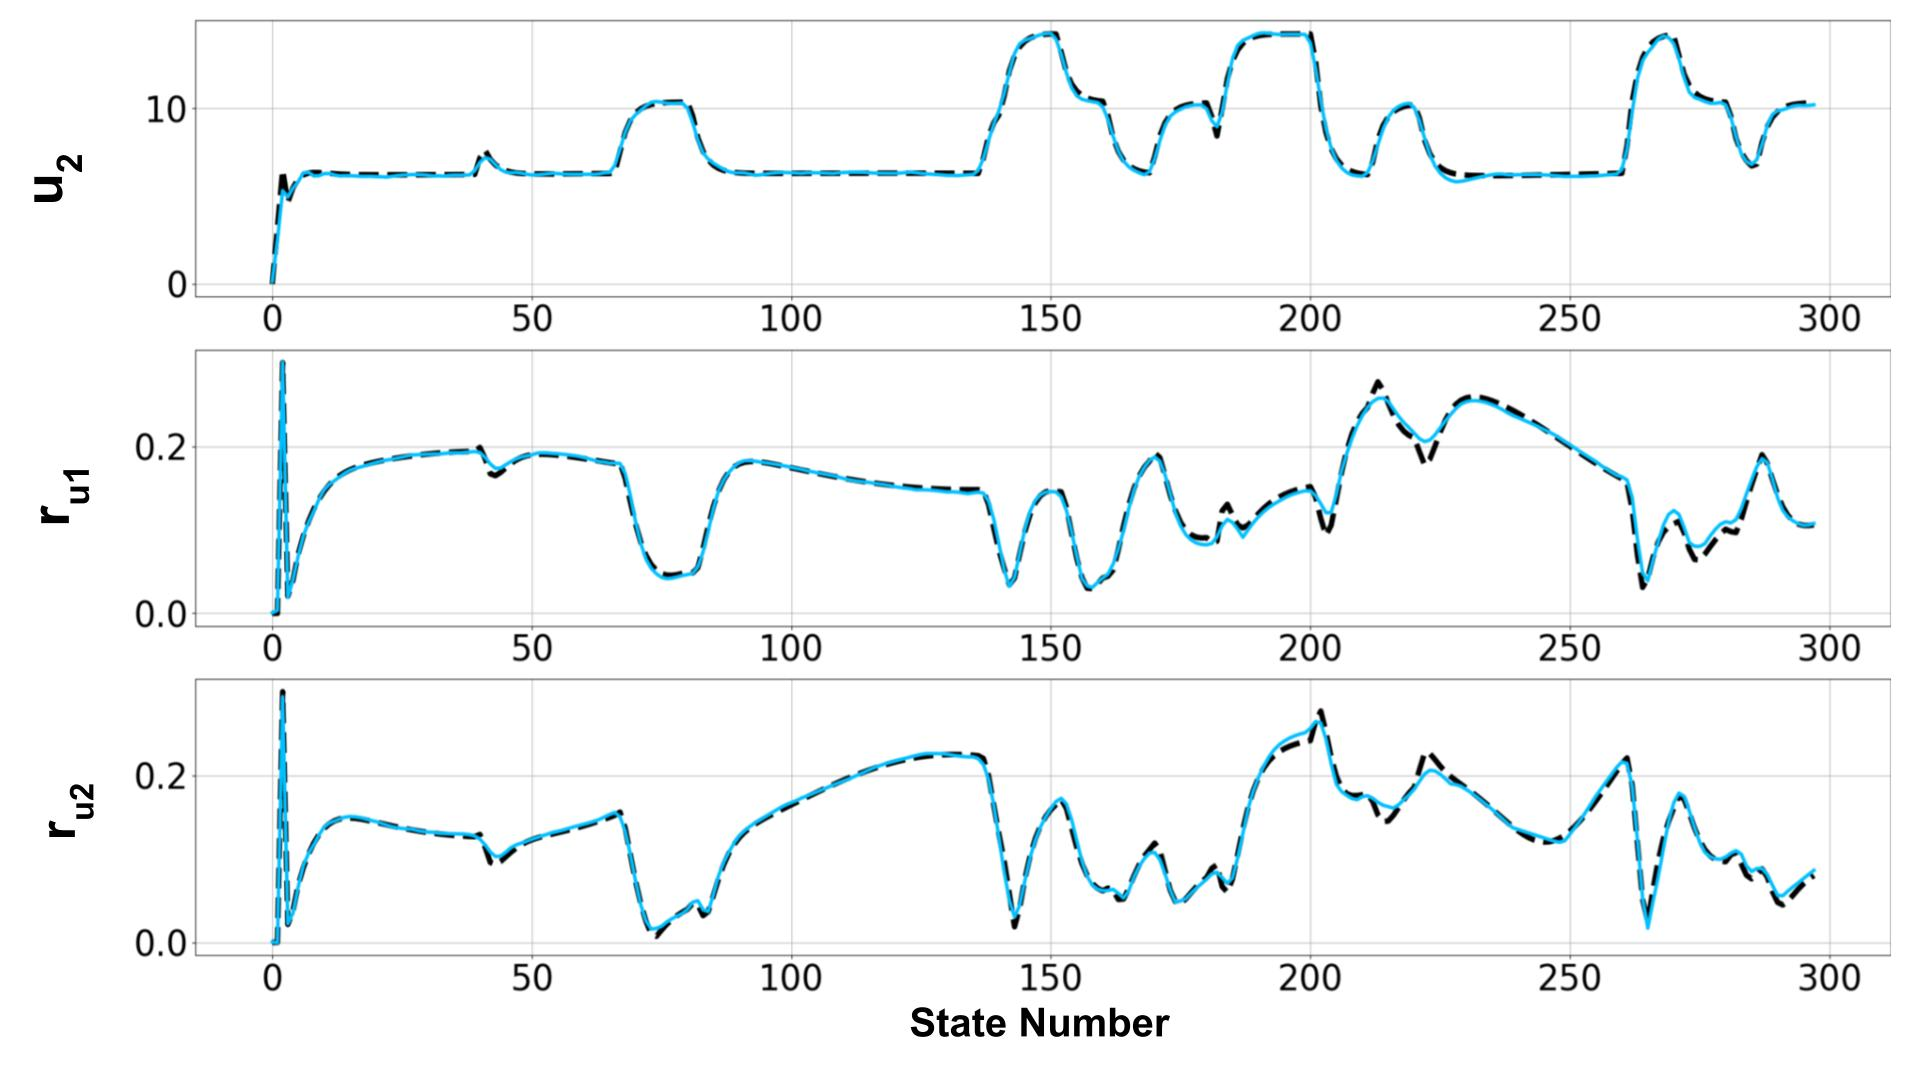
\includegraphics[width=\linewidth]{figures/learning_unic/pred_val_2_labeled.jpg}
    \end{minipage}\\
    \caption{Example of \textbf{GRU} predictions on a 300-state trajectory of the validation set. 
    Predicted outputs are displayed in blue against true values in black. $r_{x}, r_{y}$ are expressed in $m$, and control input associated values ($u_{i},r_{ui}$) are wheel angular velocities [(rad/s)].}
    \label{fig:pred_val_unic}
\end{figure}

This subsection presents qualitative results for differential drive robot.
Firstly, Figure~\ref{fig:all_models_pred_val_unic} illustrates the predictions of the \textbf{RNN}, \textbf{GRU}, \textbf{LSTM}, and \textbf{MLP} models on a 300-state trajectory from the test set.
It is noticeable that the \textbf{MLP} model provides poor accuracy, as discussed in Section~\ref{sec:nn_comparaison_unic}.
However, one can note its averaging behavior.
Additionally, the \textbf{GRU} and \textbf{LSTM} models perform similarly across all tasks, while the \textbf{RNN} shows lower performance and tends to underestimate the variations.
However, a slight resulting offset can be observed on the \textbf{GRU} and \textbf{LSTM} predictions, denoting of the slight overfitting as mentioned in Section~\ref{sec:nn_comparaison_unic} due to higher speed encountered in the test set.

However, this slight overfitting is not an issue for the proposed model application, since in the sampling-based context the trajectories encountered are more likely to match those of the validation set rather than those of the test set.
Figure~\ref{fig:pred_val_unic} shows the predictions for all output components independently, for a 300-state trajectory from the validation set.

\subsection{Quadrotor}\label{sec:nn_results_quad}

\subsubsection{Model comparison}\label{sec:nn_comparaison_quad}

\begin{table}[t]
\centering
\begin{tabular}{ | c | c  c  c | }
\hline
    \multirow{2}{*}{\textbf{Method}} & \multicolumn{3}{c|}{\textbf{Validation set}} \\ \cline{2-4}
    & \textbf{MAE$_{\Rq}$} $(m)$  & \textbf{MAE$_{\u}$} $[(rad/s)^2]$ & \textbf{MAE$_{\Ru}$} $[(rad/s)^2]$ \\ \hline
{\textbf{MLP}} & $8.9e^{-3}$ & $559.6$ & $2079.0$ \\ 
{\textbf{RNN}} & $4.5e^{-4}$ & $35.8$ & $166.4$ \\ 
{\textbf{LSTM}} & $3.1^{-4}$ & $17.7$ & $\boldsymbol{58.7}$ \\ 
{\textbf{GRU}} & $\boldsymbol{2.6e^{-4}}$ & $\boldsymbol{17.3}$ & $64.5$ \\ 
\hline
    & \multicolumn{3}{c|}{\textbf{Test set}}\\ \cline{2-4}
    & \textbf{MAE$_{\Rq}$} $(m)$  & \textbf{MAE$_{\u}$} $[(rad/s)^2]$ & \textbf{MAE$_{\Ru}$} $[(rad/s)^2]$ \\ \hline
{\textbf{MLP}} & $9.5e^{-3}$ & $608.5$ & $2050.9$ \\ 
{\textbf{RNN}} &  $1.4e^{-3}$ & $103.3$ & $544.8$ \\ 
{\textbf{LSTM}} & $1.4e^{-3}$ & $79.7$ & $308.1$ \\ 
{\textbf{GRU}} & $\boldsymbol{1.1e^{-3}}$ & $\boldsymbol{71.0}$ & $\boldsymbol{279.8}$ \\ 
\hline
    
\end{tabular}
\caption{
MAE on the $\boldsymbol{r_q}$, $\boldsymbol{u}$ and $\boldsymbol{r_u}$ components of the output vector computed on the validation and test sets for a trained RNN, GRU, and LSTM model, for the quadrotor.}
    \label{tab:NN_results_table_Q}
\end{table}

\begin{table}[t]
\centering
\begin{tabular}{ | c | c  c  c | }
\hline
    \textbf{Time (ms)} & 100 states  & 200 states & 300 states \\ \hline
    $T_{euler}$ & $26.2 \pm 1.2$ & $39.1 \pm 3.6$ & $58.7 \pm 4.9$ \\ 
$T_{dopri5}$ & $123.7 \pm 17.3$ & $255.2 \pm 17.8$ & $419.6 \pm 24.5$ \\ 
$T_{RNN}$ & $\boldsymbol{0.9} \pm 0.3$ & $\boldsymbol{1.8} \pm 0.3$ & $\boldsymbol{2.2} \pm 0.5$ \\ 
$T_{LSTM}$ & $2.5 \pm 0.3$ & $4.8 \pm 0.3$ & $7.7 \pm 0.8$ \\ 
$T_{GRU}$ & $2.1 \pm 0.2$ & $4.3 \pm 0.3$ & $5.8 \pm 0.4$  \\ \hline
\end{tabular}
\caption{
Average prediction time (ms) over 100 predictions on trajectories composed of 100 states, 200 states and 300 states, for an \textbf{RNN}, \textbf{GRU}, \textbf{LSTM}, the \textbf{Euler} integrator, and the \textbf{dopri5} integrator, for the quadrotor.}
    \label{tab:timepred}
\end{table}

Table~\ref{tab:NN_results_table_Q} reports the MAE for the different output vector components on the validation and test sets. 
First of all, note that the \textbf{MLP} again demonstrates a poor performance, as previously shown in Section~\ref{sec:nn_results_unic}, confirming the need for a recurrent neural network.
A deviation of up to 30\% from the average expected values (cf. Table~\ref{tab:datas_stats}) is observed in the validation and test sets.

Among recurrent models, \textbf{RNN} offers the least accurate predictions, with up to 7\% error on the $\boldsymbol{r_u}$ components of the test set.
On the other hand, \textbf{GRU} provides the best accuracy on all the components on both sets except for $\Ru$ on the validation set, but for which predictions remain close to expected values with less than 1\% deviation from expected mean values.
\textbf{GRU} shows the best reliability and generalizability of the trained model to unseen samples from a different distribution.
\textbf{GRU} performance on the test set shows that the predictions along $\boldsymbol{r_q}$ remain highly accurate (less than 1 millimeter average error) and that the highest errors are obtained on $\boldsymbol{r_u}$ but do not exceed 4\% of the expected average value.
The \textbf{LSTM} provides the best predictions on the $\Ru$ component of the validation set. 
However, the results show a slightly lower accuracy than \textbf{GRU} on the other components with an average error of 4.5\% on test set $\boldsymbol{r_u}$ predictions.
Nevertheless, \textbf{LSTM} is more accurate on all components than \textbf{RNN}.
Overall, \textbf{RNN} performs the worst while \textbf{GRU} and \textbf{LSTM} provide similar results, with an overall better accuracy for \textbf{GRU}.
Moreover, the latter shows a better generalization to unseen trajectories that are slightly different from the training set.

In order to choose the most advantageous model or method for computing uncertainty tubes in terms of prediction time, the methods/models are applied to trajectories of different lengths (i.e. made up of a certain number of desired states). 
Table~\ref{tab:timepred} shows the results obtained on trajectories of several hundred states. 
Note that with the current system, the number of ordinary equations solved for each element in the sequence (i.e. trajectory state) is equal to 91.
The results indicate that the average prediction time for neural networks is an order of magnitude faster compared to the \textbf{Euler} method and over ten times faster than the \textbf{dopri5} integrator. 
Additionally, the computing times for all methods exhibit an approximately linear relationship with the number of states in the trajectory.
Also note that among these models, \textbf{RNN} is the fastest to perform the predictions, which is explained by the fact that the network size is smaller than \textbf{LSTM}, and the \textbf{RNN} cell performs fewer internal operations than the \textbf{GRU} cell.
In the context of robust sampling-based motion planning, where the neural network needs to be queried tens of thousands of times for multi-state trajectories, the observed gains in computation time can become much more significant as the number of trajectories to be evaluated increases.

Finally, even if \textbf{RNN} excels in inference time when making predictions; its accuracy is noticeably lower when contrasted with that of \textbf{GRU}.
As for the \textbf{LSTM}, it provides the slowest inference time and less accurate predictions than the \textbf{GRU}, except for the $\Ru$ component of the validation set.
Additionally, its hidden state implementation results in twice as many parameters having to be saved per sampling-based motion planner iteration compared to \textbf{GRU}, which translates by a higher memory cost when growing trees or graphs with thousands of nodes.
Therefore, based on the model implementation details and results presented above, the use of \textbf{GRU} is recommended in the context of a sampling-based motion planner for the quadrotor application.
Indeed, the latter is much faster than methods based on \myglsentry{odes} solvers while offering the most accurate predictions, thus offering the best trade-off between inference time and accuracy.

\subsubsection{Ablation study}

\begin{table*}[h!]
    \centering
    \begin{tabular}{ | c | c  c  c | }
    \hline
    \multirow{2}{*}{\textbf{Method}} & \multicolumn{3}{c|}{\textbf{Validation set}} \\ \cline{2-4}
        & \textbf{MAE$_{\Rq}$} $(m)$  & \textbf{MAE$_{\u}$} $[(rad/s)^2]$ & \textbf{MAE$_{\Ru}$} $[(rad/s)^2]$ \\ \hline
    {\textbf{GRU$\boldsymbol{_V}$}} & $\boldsymbol{2.5e^{-4}}$ & $25.2$ & $74.6$ \\
    {\textbf{GRU$\boldsymbol{_A}$}} & $2.6e^{-4}$ & $17.9$ & $77.6$ \\
    {\textbf{GRU$_{\boldsymbol{V A}}$}} & $2.6e^{-4}$ & $\boldsymbol{17.3}$ & $\boldsymbol{64.5}$ \\
    \hline
        & \multicolumn{3}{c|}{\textbf{Test set}}\\ \cline{2-4}
        & \textbf{MAE$_{\Rq}$} $(m)$  & \textbf{MAE$_{\u}$} $[(rad/s)^2]$ & \textbf{MAE$_{\Ru}$} $[(rad/s)^2]$ \\ \hline
    {\textbf{GRU$\boldsymbol{_V}$}} & $\boldsymbol{1.0e^{-3}}$ & $92.8$ & $365.6$ \\
    {\textbf{GRU$\boldsymbol{_A}$}} &  $1.3e^{-3}$ & $82.7$ & $418.5$ \\
    {\textbf{GRU$_{\boldsymbol{V A}}$}} & $1.1e^{-3}$ & $\boldsymbol{71.0}$ & $\boldsymbol{279.8}$ \\
    \hline
        
    \end{tabular}
    \caption{
        Quadrotor application: Results of the ablation study measured in term of MAE on the $\boldsymbol{r_q}$, $\boldsymbol{u}$ and $\boldsymbol{r_u}$ components of the output vector. $V, A$ refer to the different inputs considered (linear and angular velocities, accelerations respectively). The presence of one as a subscript to the \textbf{GRU} model means that it is used as an input (e.g. $\boldsymbol{GRU_{A}}$ takes as input the acceleration only).}
     \label{tab:ablation}
\end{table*}

In theory, all the inputs to our neural network are needed by the controller and the uncertainty tubes computation methods to obtain the desired outputs. 
In order to confirm this for the neural network as well, an ablation study is conducted on the \textbf{GRU} model to show that the choice of input vector components described in Section~\ref{sec:quad_nn_architecture} is the most relevant for the quadrotor case. 
The components considered for the study are the desired linear and angular velocities, and the desired accelerations, denoted $V$ and $A$ respectively. 
The proposed model takes both inputs and is denoted \textbf{GRU$\boldsymbol{_{VA}}$}. 
Two ablations are defined, one for each input, resulting in two models: \textbf{GRU$\boldsymbol{_V}$} which takes as input the linear and angular velocities only, and \textbf{GRU$\boldsymbol{_A}$} which only takes the accelerations as input. 
Each model is trained in the same way detailed in Section~\ref{sec:train_quad} and is evaluated according to the MAE metrics described in Section~\ref{sec:metric}.

Note that since the network is intended to be used in a sampling-based approach, no ablation study is performed on the output vector since our objective is to use a single model within the planner, keeping the memory and computational costs low.

Table~\ref{tab:ablation} provides the results of the ablation study.
Results show that each input component specializes in predicting one of the desired outputs.
Specifically, the model \textbf{GRU$\boldsymbol{_V}$} using the velocity component only yields accurate results for $\Rq$ and $\Ru$ on both the validation and test sets, while the one solely using the accelerations leads to accurate results on $\u$ on both sets.

These outcomes are expected since $\Rq$ depends indirectly on the state of the robot $\q$ only, which can be inferred from the velocities easily. 
On the other hand, the inner workings of the chosen controller give more importance to the accelerations of the robot, while the velocities are used for computing internal errors. T
his explains the fact that \textbf{GRU$\boldsymbol{_A}$} yields good results for the $\u$ predictions.

On the other hand, Table~\ref{tab:ablation} shows an improvement on both the control inputs $\u$ and the control uncertainty tubes $\Ru$ using both the velocities and the accelerations as inputs to the neural network. 
Indeed, even though a slight degradation can be noted in the performance of $\Rq$ predictions, \textbf{GRU$\boldsymbol{_{VA}}$} achieves the best overall results on both the validation and test sets, thus justifying the implementation of Section~\ref{sec:architecture}. 
This can be explained by the fact that the output values are not related to the input components independently, they also depend on the interactions between these variables. 
Also, remind that the chosen controller and uncertainty tubes computation methods use both the velocities and the accelerations of the robot to obtain the desired outputs.

Note that the results of this ablation study are specific to the chosen case of the quadrotor/controller.
Another dynamical system might need a different set of inputs to obtain accurate predictions.

\subsubsection{Qualitative results}

\begin{figure}[htp]
    \centering
    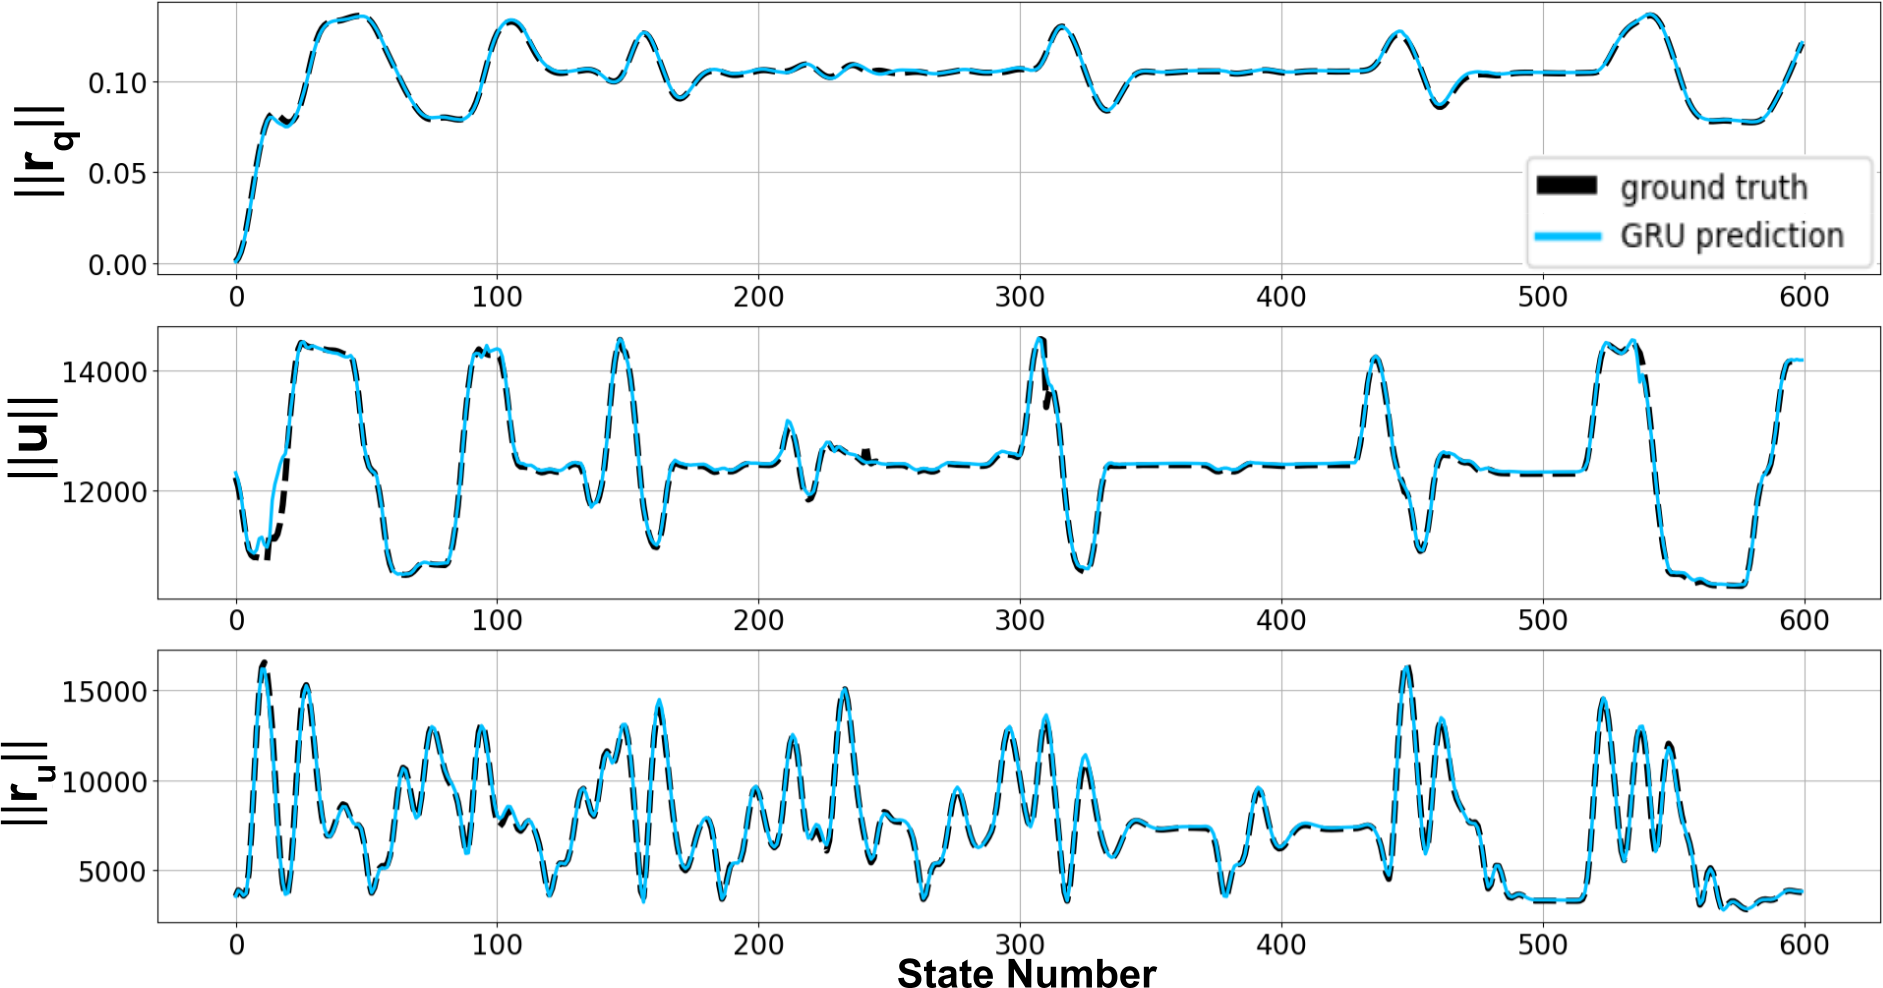
\includegraphics[width=0.99\linewidth]{figures/learning_quadrotor/long_pred.png}
    \caption{Example of \textbf{GRU} predictions on a 600-state trajectory generated in the same way as the test set. $||\Rq||, ||\u||$ and $||\Ru||$ refer to the norm of their respective vector. Predicted outputs are displayed in blue against true values in black. $||\Rq||$ is expressed in $m$, and control input associated values ($||\u||,||\Ru||)$ are squared propeller angular velocities [(rad/s)²].}
    \label{fig:long_test}
\end{figure}

\begin{figure}[htp]
    \centering
    \begin{minipage}{0.49\linewidth}
        \centering
        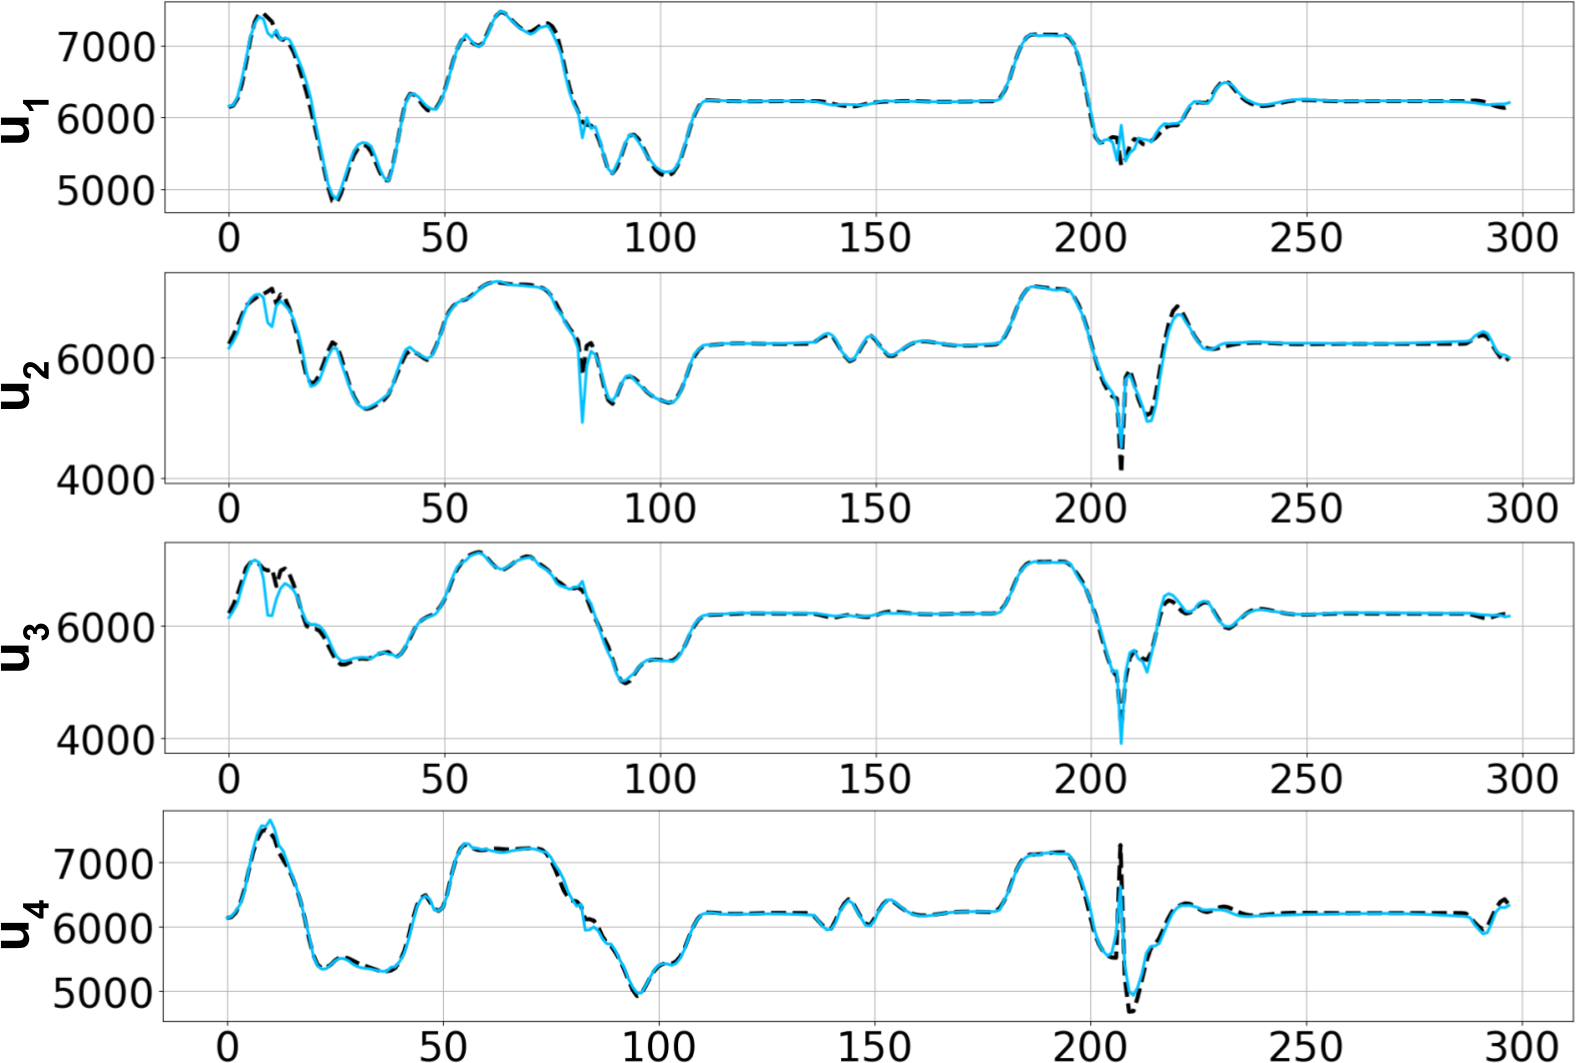
\includegraphics[width=\linewidth]{figures/learning_quadrotor/pred_u.jpg}\\
        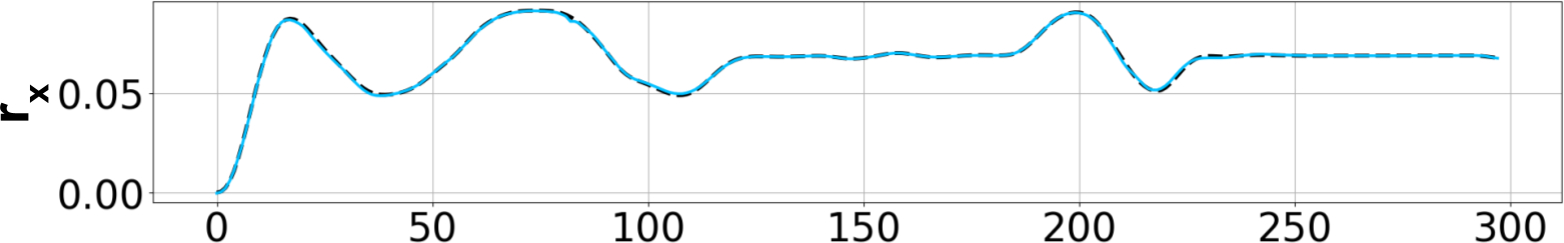
\includegraphics[width=\linewidth]{figures/learning_quadrotor/pred_rx.jpg}
    \end{minipage}
    \begin{minipage}{0.49\linewidth}
        \centering
        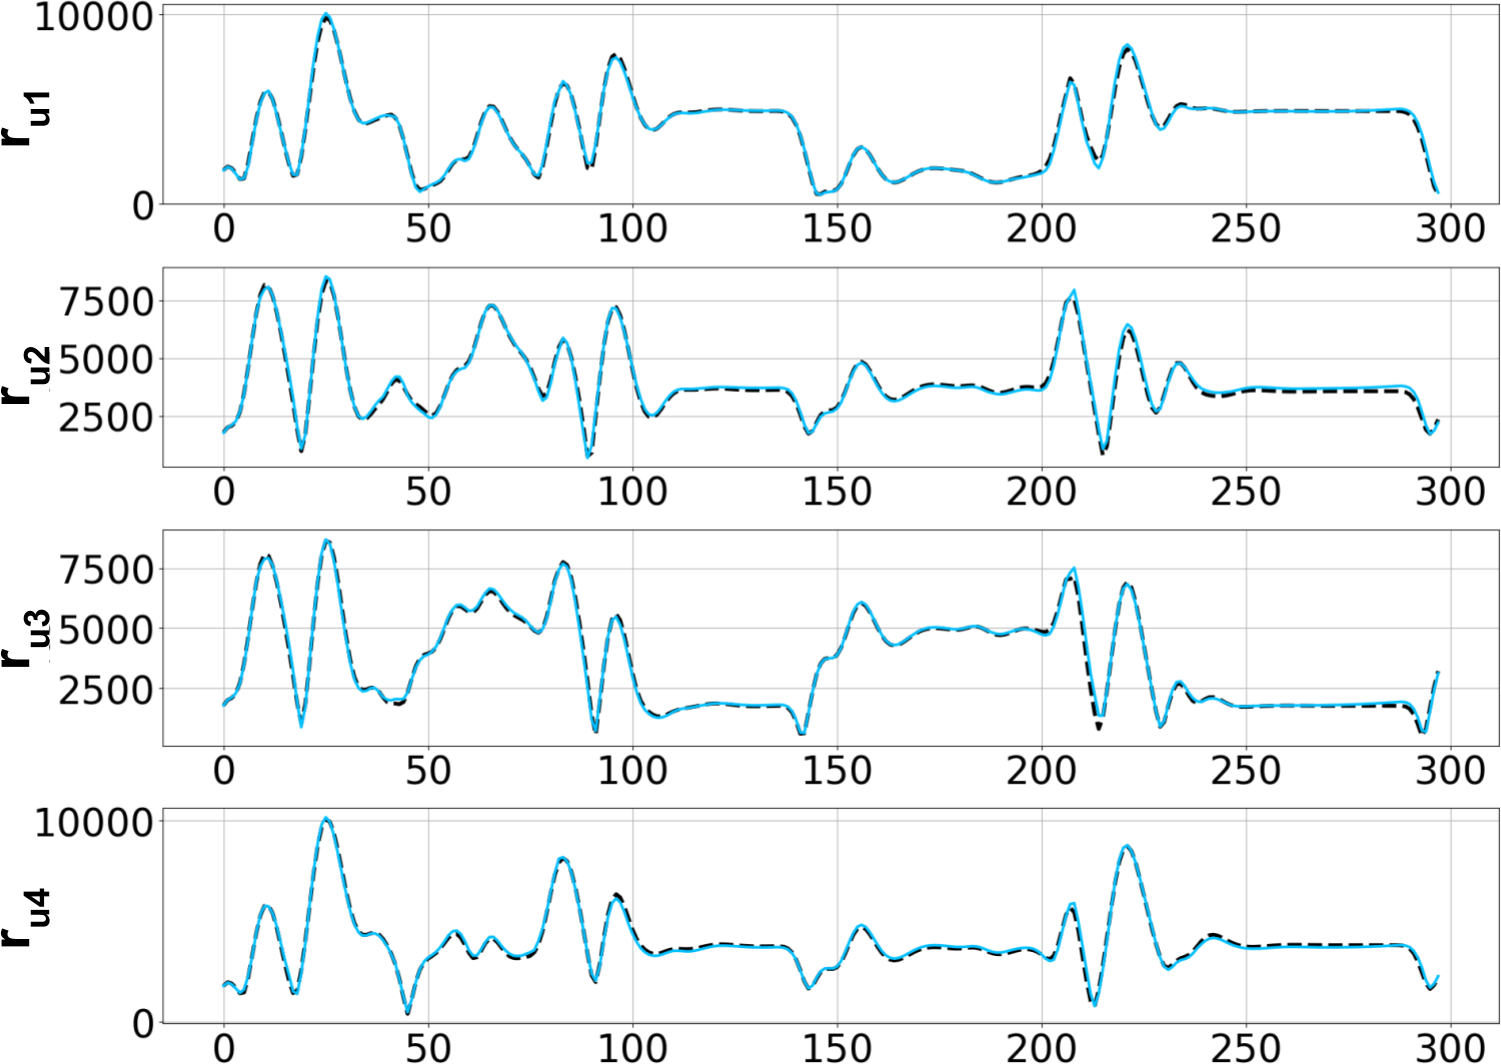
\includegraphics[width=\linewidth]{figures/learning_quadrotor/pred_ru.jpg}\\
        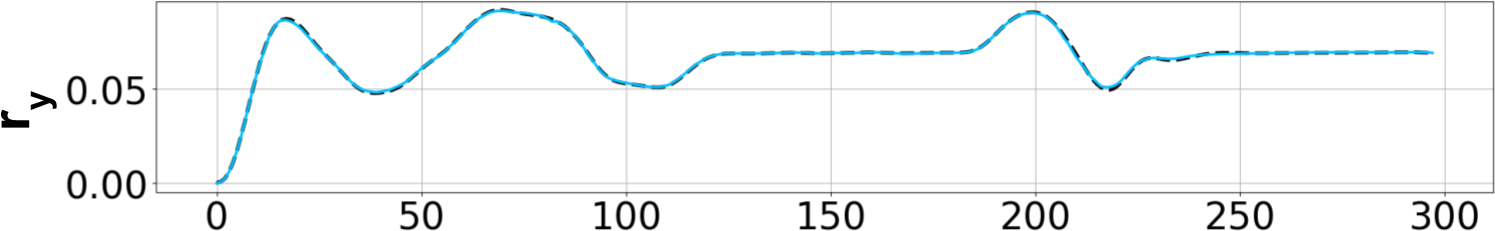
\includegraphics[width=\linewidth]{figures/learning_quadrotor/pred_ry.jpg}
    \end{minipage}\\
    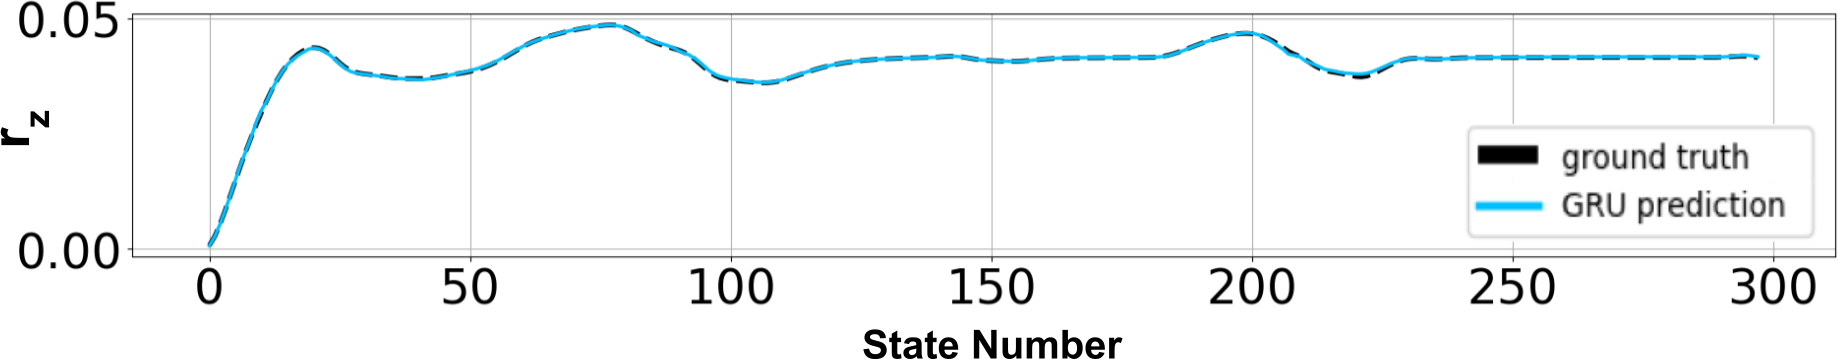
\includegraphics[width=0.49\linewidth]{figures/learning_quadrotor/pred_rz.jpg}
    \caption{Example of \textbf{GRU} predictions on a 300-state trajectory of the test set. 
    Predicted outputs are displayed in blue against true values in black. $r_{x}, r_{y}, r_{z}$ are expressed in $m$, and control input associated values ($u_{i},r_{ui}$) are squared propeller angular velocities [(rad/s)²].}
    \label{fig:pred_test}
\end{figure}

\begin{figure}[b]
    \centering
    \includesvg[width=0.99\linewidth]{figures/learning_quadrotor/all_models.svg} 
    \caption{Comparison of predictions obtained using the different recurrent neural network architectures as well as the \textbf{MLP} on a 300-state trajectory of the test set. $||\Rq||, ||\u||$ and $||\Ru||$ refer to the norm of their respective vector. 
    True values are displayed in black, \textbf{GRU} predictions in blue, \textbf{MLP} predictions in purple, \textbf{LSTM} outputs in yellow, and basic \textbf{RNN} predictions are in red.}
    \label{fig:MLP_pred_val}
\end{figure}

\begin{figure}[b]
    \centering
    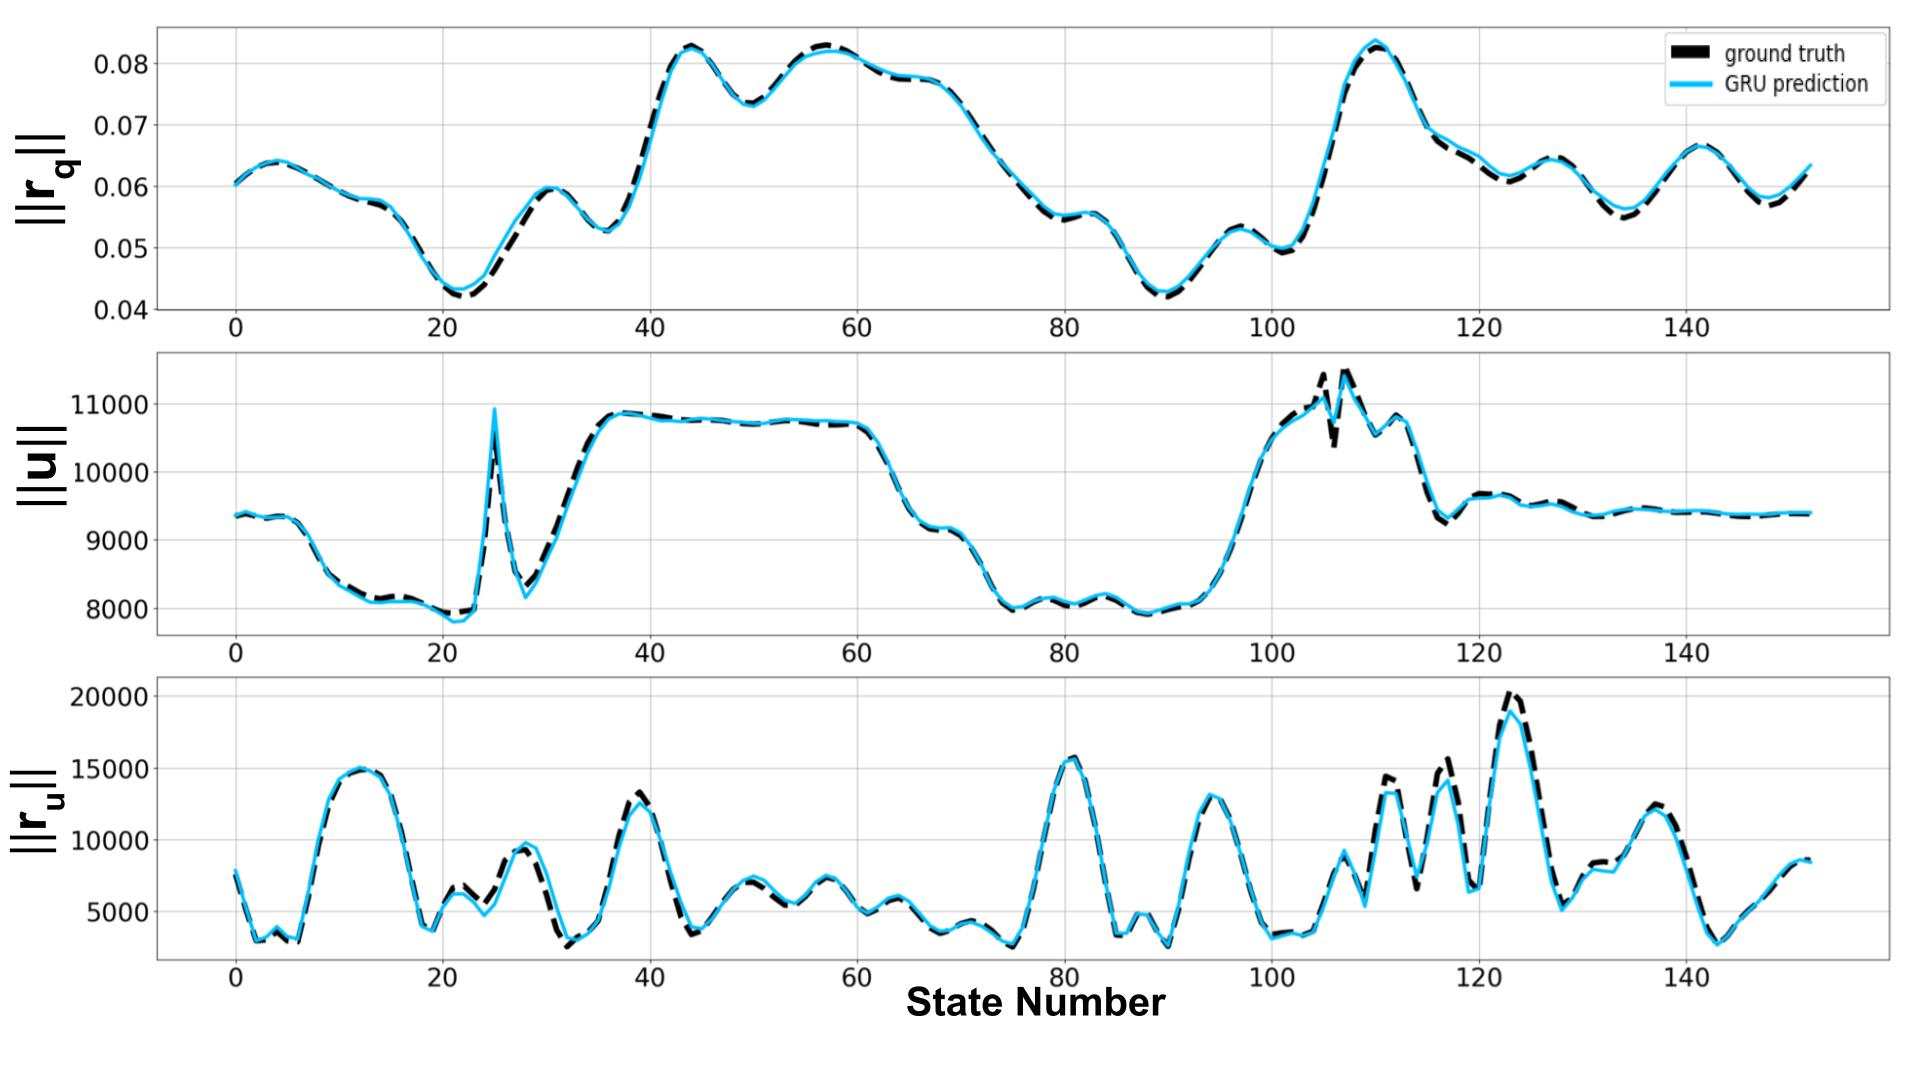
\includegraphics[width=0.99\linewidth]{figures/learning_quadrotor/non_zero_hidden.jpg} 
    \caption{Example of \textbf{GRU} predictions on a 150-state trajectory of the test set starting from a non-zero hidden state.
    $||\Rq||, ||\u||$ and $||\Ru||$ refer to the norm of their respective vector. 
    True values are displayed in black and \textbf{GRU} predictions in blue.}
    \label{fig:non_zero_hidden}
\end{figure}

The robust generalization of the \textbf{GRU} model to the test set is highlighted in Figure~\ref{fig:pred_test}, depicting predictions for all the components of the output vector for a trajectory composed of 300 states (i.e. $T_F=15s$).
One can observe larger prediction errors during transient phases involving the higher velocities present in the test set than in the training one.
Note that the neural network predictions in these phases have a moving average `behavior'. 
However, an overall good fitting of the predictions can be highlighted.

In addition to the results discussed in Section~\ref{sec:nn_comparaison_quad}, Figure~\ref{fig:MLP_pred_val} shows an example of \textbf{MLP}'s inability to provide accurate predictions on a 300-state test set trajectory, with a tendency to simply average expected values over the latter.
In comparison, the \textbf{GRU} model is able to accurately predict the control inputs and the uncertainty tube across the whole trajectory. 
Also note a close performance between \textbf{GRU} and \textbf{LSTM} on all tasks, while \textbf{RNN} lags behind and tends to underestimate large variations of control uncertainty tubes $\Ru$.

In order to show the stability of the proposed method, Figure~\ref{fig:long_test} depicts the norm of predicted vectors for a 600-state trajectory generated in the same way as the test set but considering a total length of 30s (i.e. $T_F=30s$).
Note that this trajectory is twice as long as those used in training, validation and test sets.
The results show the same behavior in transient phases where higher velocities are encountered.
However, one can observe that the model is consistent throughout longer sequences even with a different distribution from the one it was trained one. 

Finally, Figure~\ref{fig:non_zero_hidden} highlights the ability of the proposed model to provide predictions with good accuracy when starting from non-zero hidden state. 
This is convenient in a sampling-based motion planning context, where successive local trajectories must be evaluated.
Note that, in the dataset all trajectories start from a hovering state (i.e., null velocities and accelerations). 
Hence, in order to generalize to trajectories where initial velocities and accelerations are not null one can simply append a planned sub-trajectory arriving at this initial state and starting from the hovering state.

\section{Conclusion} \label{sec:NN_concl}

This chapter has presented a \textbf{GRU}-based neural network architecture to predict uncertainty tubes and control inputs along sequences of desired states for any dynamical system.
Results on a quadrotor and differential drive robot use cases show that leveraging recurrent neural network architectures is of key importance due to the temporal dependency of the predictions.
Furthermore, it has been shown that a \textbf{GRU} is more appropriate in a sampling-based tree planner context than \textbf{RNN} or \textbf{LSTM} as it proposes the best compromise between prediction accuracy, generalizability, inference time and memory cost.
By directly correlating the inputs and outputs of the neural network, the proposed predictor $\boldsymbol{g}$ eliminates the need for sequential computation inherent in the \myglsentry{odes} addressed in this thesis. 
This design simplifies the process and reduces the computational burden, making it more efficient than the traditional \myglsentry{odes} framework while maintaining a good accuracy.

Additionally, great care was taken to develop a learning process that ensures the learned models are independent of the environment, enabling their application to motion planning problems. 
However, the GRU-based approach still relies on robot model parameters, such as system nominal parameters and controller gains. 
To further address these dependencies, future investigations could explore strategies such as:
\begin{itemize}
    \item GPU acceleration; a technique that leverage massive parallelization thanks to computational power of modern GPUs.
    \item Transfer learning; a method that allows a model to apply knowledge gained from one task or dataset to a new, related task, reducing the need for extensive retraining.
    \item Ensemble learning; a technique that involves combining multiple models to improve prediction accuracy and generalized performance.
\end{itemize}

Despite these potential areas for improvement, the remainder of this thesis will focus on incorporating the GRU-based architecture into sampling-based motion planners to plan robust robot motions against parametric uncertainties in a more efficient way than what was proposed in Chapter~\ref{chap:samp}.
